\chapter{Application of the Calculus of Variations to Eigenvalue Problems}

In the preceding chapter we saw that eigenvalue problems of differential equations are closely connected with those of quadratic forms. As a matter of fact, these eigenvalue problems correspond to the problem of transforming a quadratic form in infinitely many variables to principal axes.

If, for example, we denote the potential and kinetic energies of a one-dimensional continuum by
\[
U=\frac12\int_0^\pi p\left(\frac{\partial u}{\partial x}\right)^2dx
\qquad\text{and}\qquad
T=\frac12\int_0^\pi \rho\left(\frac{\partial u}{\partial t}\right)^2dx,
\]
we need only write $u=\sum_{\nu=1}^{\infty}f_\nu(t)\sin \nu x$ and expand $p$ and $\rho$ in Fourier series; then we can consider the two expressions $U$ and $T$ as quadratic forms in the infinitely many variables (coordinates) $f_\nu$ and $\dot f_\nu$, respectively. If an orthogonal transformation
\[
f_\nu=\sum_{\mu=1}^{\infty}l_{\nu\mu}q_\mu,
\qquad
\dot f_\nu=\sum_{\mu=1}^{\infty}l_{\nu\mu}\dot q_\mu,
\qquad (\nu=1,2,\ldots)
\]
of these variables into new variables $q_\nu$ and $\dot q_\nu$ can be determined in such a way that $U$ and $T$ take the form
\[
U=\sum_{\nu=1}^{\infty}\lambda_\nu q_\nu^2,
\qquad
T=\sum_{\nu=1}^{\infty}\dot q_\nu^2,
\]
then the numbers $\lambda_\nu$ are the eigenvalues of our vibration problem. Since the eigenvalues of a quadratic form are characterized by simple extremum properties, it seems reasonable to consider a similar characterization for the case of quadratic functionals. However, instead of treating these functionals as limits of finite quadratic forms of a finite number of variables, we shall formulate and apply the extremum properties in question directly without referring to such a limit process.

\section{Extremum Properties of Eigenvalues}
\subsection{Classical Extremum Properties}
Consider the eigenvalue problem of a self-adjoint second order partial differential equation
\begin{equation}\tag{1}
L[u]+\lambda\rho u=(pu_x)_x+(pu_y)_y-qu+\lambda\rho u=0
\qquad (p>0,\ \rho>0);
\end{equation}
here $x$ and $y$ are independent variables in the fundamental domain $G$, bounded by one or several continuous curves with piecewise continuous tangents. Let the boundary condition have the form $u=0$, or in general $\partial u/\partial n+\sigma u=0$, where $\sigma$ denotes a piecewise continuous function of position on the boundary $\Gamma$ and $\partial/\partial n$ differentiation in the direction of the outer normal.\footnote{It should be stated that in general this boundary condition must be interpreted in the ``weak'' sense; i.e., the function is not actually required to assume boundary values everywhere on $\Gamma$. This delicate point will be fully discussed in Vol. II, Ch. VII in connection with the existence proof. Here, where we assume the existence of the solutions, we need not specify the behavior of $u$ at the boundary.} Typical quadratic functional expressions for the variational eigenvalue problems are:
\begin{equation}\tag{2}
\mathfrak D[\varphi]=D[\varphi]+\int_\Gamma p\sigma\varphi^2\,ds
\end{equation}
with
\begin{equation}\tag{2a}
D[\varphi]=\iint_G p(\varphi_x^2+\varphi_y^2)\,dx\,dy+\iint_G q\varphi^2\,dx\,dy
\end{equation}
and
\begin{equation}\tag{3}
H[\varphi]=\iint_G \rho\varphi^2\,dx\,dy;
\end{equation}
the associated polar forms
\[
\mathfrak D[\varphi,\psi]=D[\varphi,\psi]+\int_\Gamma p\sigma\varphi\psi\,ds,
\]
\[
D[\varphi,\psi]=\iint_G p(\varphi_x\psi_x+\varphi_y\psi_y)\,dx\,dy+\iint_G q\varphi\psi\,dx\,dy,
\]
\[
H[\varphi,\psi]=\iint_G \rho\varphi\psi\,dx\,dy
\]
satisfy the relations
\[
\mathfrak D[\varphi+\psi]=\mathfrak D[\varphi]+2\mathfrak D[\varphi,\psi]+\mathfrak D[\psi],
\]
\[
H[\varphi+\psi]=H[\varphi]+2H[\varphi,\psi]+H[\psi].
\]
We require the argument function $\varphi$ to be continuous in $G+\Gamma$ and to have piecewise continuous first derivatives in $G$.

Here piecewise continuity of a function $\psi$ in $G$ means: $G$ may be subdivided into a finite number of regions $G_1,G_2,\ldots,G_m$ by arcs with piecewise continuous tangents such that $\psi$ is continuous in each closed subregion of $G$ not containing any of these arcs in its interior.

If the boundary condition $u=0$ is prescribed, then $u$ is assumed to be continuous in the closed region $G+\Gamma$ and to vanish on $\Gamma$.

We obtain the eigenvalues $\lambda_\nu$ and the associated eigenfunctions $u_\nu$ of the differential equation (1) from the following minimum properties: \emph{The admissible function which minimizes the expression $\mathfrak D[\varphi]$ under the condition $H[\varphi]=1$ is an eigenfunction $u_1$ for the differential equation (1) and satisfies the natural boundary condition $\partial\varphi/\partial n+\sigma\varphi=0$; the minimum value of $\mathfrak D$ is the corresponding eigenvalue. If we impose not only the condition}
\begin{equation}\tag{3a}
H[\varphi]=1
\end{equation}
\emph{but also the orthogonality condition}
\[
H[\varphi,u_1]=0,
\]
\emph{then the solution is again an eigenfunction $u_2$ of (1) satisfying the same boundary condition, and the minimum value $\mathfrak D[u_2]=\lambda_2$ is the associated eigenvalue. The successive minimum problems, $\mathfrak D[\varphi]=$ minimum subject to the condition $H[\varphi]=1$ and to the auxiliary conditions}
\[
H[\varphi,u_i]=0\qquad(i=1,2,\ldots,\nu-1),
\]
\emph{define the eigenfunctions $u_\nu$ of equation (1) with the boundary condition $\partial\varphi/\partial n+\sigma\varphi=0$; the associated eigenvalue $\lambda_\nu$ equals the minimum value $\mathfrak D[u_\nu]$.}

We can omit the normalizing condition $H[\varphi]=1$ by minimizing the quotients $\mathfrak D[\varphi]/H[\varphi]$; then the solution is determined only up to an arbitrary factor of proportionality.

If the boundary condition is $u=0$, the same variational problems define eigenvalues and eigenfunctions; but the boundary condition $\varphi=0$ is now added to the admissibility conditions. Then the boundary term $\int_\Gamma p\sigma\varphi^2\,ds$ in $\mathfrak D[\varphi]$ drops out automatically.

A proof that our minimum problem does possess solutions with continuous second derivatives will be given in Volume II, in connection with the direct methods of the calculus of variations. At present we proceed on the assumption that minimum problems of the above type possess solutions.

We have to show (a) that the solutions of the variational problem are also eigenfunctions for our differential equation problem, and (b) that they furnish all the eigenfunctions. The second assertion will be proved in \S3 by showing that the system of functions $u_1,u_2,\ldots$ obtained from the variational problem is complete. Statement (a) could be derived from the general multiplier rule of Ch. IV, \S7 but will now be obtained directly.

Let us begin with the first variational problem, and assume that its solution $u_1$ satisfies the condition $H[u_1]=1$. If $\zeta$ is any function which satisfies the same conditions as $\varphi$, and if $\epsilon$ is an arbitrary constant, then for every value of $\epsilon$ and for $u=u_1$, $\lambda=\lambda_1$ we have
\[
\mathfrak D[u+\epsilon\zeta]\ge\lambda H[u+\epsilon\zeta]
\]
or
\[
2\epsilon\left\{\mathfrak D[u,\zeta]-\lambda H[u,\zeta]
+\frac{\epsilon}{2}(\mathfrak D[\zeta]-\lambda H[\zeta])\right\}\ge0;
\]
these statements are equivalent in view of the relation $\mathfrak D[u]=\lambda H[u]$. The second inequality can be valid for arbitrary values of $\epsilon$ only if equation
\begin{equation}\tag{4}
\mathfrak D[u,\zeta]-\lambda H[u,\zeta]=0
\end{equation}
holds, i.e. if the first variation of the expression $\mathfrak D-\lambda H$ vanishes.

We now transform the expression $\mathfrak D[u,\zeta]$ according to Green's formula
\[
\mathfrak D[u,\zeta]=-
\iint_G \zeta L[u] \,dx\,dy
+\int_\Gamma p\sigma\zeta u\,ds
+\int_\Gamma p\zeta\frac{\partial u}{\partial n}\,ds
\]
(cf. Ch. V, \S1); since the function $\zeta$ is arbitrary, we immediately obtain equation (1) for $u=u_1$ and $\lambda=\lambda_1$. Considering the second minimum problem with the additional condition $H[\varphi,u_1]=0$, we obtain equation (4) for $u=u_2$ and $\lambda=\lambda_2$ at first only under the assumption that $\zeta$ satisfies relation
\begin{equation}\tag{5}
H[\zeta,u_1]=0.
\end{equation}
Now if $\eta$ is any function having piecewise continuous derivatives of second order, we can determine a number $t$ in such a way that the function $\zeta=\eta+tu_1$ satisfies condition (5)--we set $t=-H[u_1,\eta]$. Moreover, we note that we can, in particular, substitute the function $\zeta=u_2$ in equation (4) with $u=u_1$ and $\lambda=\lambda_1$; since $u_2$ satisfies the additional condition
\begin{equation}\tag{6}
H[u_2,u_1]=0
\end{equation}
we immediately obtain
\begin{equation}\tag{7}
\mathfrak D[u_2,u_1]=0.
\end{equation}
If we substitute our function $\zeta=\eta+tu_1$ in equation (4), writing $u=u_2$, $\lambda=\lambda_2$, we find
\[
\mathfrak D[u,\eta]-\lambda H[u,\eta]
+t(\mathfrak D[u,u_1]-\lambda H[u,u_1])=0
\]
or, taking into consideration equations (6) and (7),
\begin{equation}\tag{4a}
\mathfrak D[u,\eta]-\lambda H[u,\eta]=0.
\end{equation}
In other words, equation (4) holds also for arbitrary functions $\eta$ or $\zeta$ without regard to the auxiliary condition (5). From this it follows directly, as above, that equation (1) is valid for $u=u_2$ and $\lambda=\lambda_2$. Continuing in this way, we conclude that the eigenvalue equation (4a) holds generally for the solutions $u_i$ and the minimum values $\lambda_i$. For the solutions of the problem, which are normalized in accordance with (3a), we have the relations
\begin{equation}\tag{8}
\begin{gathered}
\mathfrak D[u_i]=\lambda_i,\qquad \mathfrak D[u_i,u_k]=0,\\
H[u_i]=1,\qquad H[u_i,u_k]=0\qquad(i\ne k).
\end{gathered}
\end{equation}
The eigenvalues thus obtained satisfy the inequality
\begin{equation}\tag{9}
\lambda_{\nu-1}\le\lambda_\nu,
\end{equation}
since the class of functions $\varphi$ admissible in the problem characterizing $\lambda_\nu$ is a subset of the corresponding class admissible in the previous problem characterizing $\lambda_{\nu-1}$. Thus the minimum $\lambda_\nu$ can be no smaller than the preceding minimum $\lambda_{\nu-1}$.

Our variational problems produce an infinite sequence of eigenvalues and eigenfunctions of the associated differential equation problem. Conversely, the eigenvalues and eigenfunctions associated with the differential equation are obtained as solutions of our variational eigenvalue problems, as will be shown in \S3, 1.

\subsection{Generalizations}
It need hardly be pointed out that the other eigenvalue problems considered in the preceding chapter can also be treated from the standpoint of the calculus of variations.\footnote{See Courant, \"Uber die Anwendung der Variationsrechnung.\ldots} This is equally true of single and multiple integrals and of differential equations of second and higher order. For example, the eigenvalue problem of the Sturm--Liouville equation
\[
(pu')'-qu+\lambda\rho u=0
\]
with the boundary conditions $u'(0)-h_1u(0)=u'(\pi)+h_2u(\pi)=0$ corresponds to a variational problem of the form
\[
\mathfrak D[\varphi]=\int_0^\pi(p\varphi'^2+q\varphi^2)\,dx
+h_1p(0)\varphi(0)^2+h_2p(\pi)\varphi(\pi)^2=\min.
\]
without boundary conditions. All the homogeneous boundary conditions previously listed can be obtained by an appropriate choice of $h_1$ and $h_2$, if we consider the boundary conditions $u(0)=u(\pi)=0$ as limiting cases for infinite $h_1$ and $h_2$.

Even for Sturm--Liouville equations with singularities at end points, the eigenvalues and eigenfunctions may be characterized by variational problems. It will suffice to give the formulation for Legendre polynomials and for Bessel functions. We obtain the Legendre polynomials by considering the free problem with
\[
\mathfrak D[\varphi]=\int_{-1}^{+1}(1-x^2)\varphi'^2\,dx,
\qquad
H[\varphi]=\int_{-1}^{+1}\varphi^2\,dx;
\]
here both end points are singular. The Bessel function $J_0(x\sqrt\lambda)$ of order zero arises from the problem for which
\[
\mathfrak D[\varphi]=\int_0^1x\varphi'^2\,dx,
\qquad
H[\varphi]=\int_0^1x\varphi^2\,dx
\]
with no boundary condition at $x=0$, the Bessel functions of $m$-th order with $m\ge1$ from the problem for which
\[
\mathfrak D[\varphi]=\int_0^1\left(x\varphi'^2+\frac{m^2}{x}\varphi^2\right)dx,
\qquad
H[\varphi]=\int_0^1x\varphi^2\,dx
\]
with the boundary condition $\varphi(0)=0$. The boundary condition $\varphi(1)=0$ at the regular end point $x=1$ is associated with the problem of a clamped membrane.

Analogous results are obtained for self-adjoint differential equations of higher order in more dimensions, such as the equation of the vibrating plate,
\begin{equation}\tag{10}
\Delta\Delta u-\lambda u=0.
\end{equation}
To treat the problem of a clamped plate (cf. Ch. IV, \S10) we set
\[
\mathfrak D[\varphi]=D[\varphi]=\iint_G(\Delta\varphi)^2\,dx\,dy,
\qquad
H[\varphi]=\iint_G\varphi^2\,dx\,dy
\]
and impose the condition
\[
\varphi=\frac{\partial\varphi}{\partial n}=0
\]
on the boundary $\Gamma$ of $G$. With these conventions the rest of the discussion and the formulas of subsection 1 remain entirely unchanged.

Other types of eigenvalue problems, not treated explicitly in Chapter V, immediately fit into the scheme presented here. If we recall that $\tfrac12H[\varphi]$ corresponds to the kinetic energy of our continuum with mass density $\rho$, while $\tfrac12\mathfrak D[\varphi]$ represents the potential energy, it is natural to construct mechanical models in which the mass is not only distributed continuously over the domain $G$ but concentrated at isolated points. For models of this kind we obtain (in one dimension) the expression
\begin{equation}\tag{11}
\mathfrak H[\varphi]=\int_G\rho\varphi^2\,dx+\sum_{\nu=1}^h b_\nu\varphi(x_\nu)^2
\end{equation}
which takes the place of $H$; here $x_1,x_2,\ldots,x_h$ denote given points in the domain $G$ and the numbers $b_\nu$ are given constants. A quadratic functional of this form corresponds to the assumption that masses of magnitude $b_\nu$ are concentrated at the points $x_1,x_2,\ldots,x_h$. We shall assume throughout that these masses are non-negative. Similarly, we can consider more general expressions of the form
\begin{equation}\tag{12}
\mathfrak D[\varphi]=\int_Gp\varphi'^2\,dx+\int_Gq\varphi^2\,dx+\sum_{\nu=1}^h a_\nu\varphi(x_\nu)^2.
\end{equation}
For such problems we find eigenvalues and eigenfunctions using precisely the same notation and argument as in subsection 1. These eigenfunctions satisfy the differential equation
\begin{equation}\tag{13}
L[u]+\lambda\rho u=(pu')'-qu+\lambda\rho u=0
\end{equation}
except at the points $x_1,x_2,\ldots,x_h$, where natural boundary and \emph{jump conditions} for the derivatives occur. We obtain these conditions immediately by forming the first variation. The eigenfunctions of our problem, multiplied by $\sqrt\rho$, are no longer orthogonal; instead, they satisfy the conditions\footnote{H. Kneser has suggested the term ``weighted orthogonality.''}
\begin{equation}\tag{14}
\int_G\rho u_i u_j\,dx+\sum_{\nu=1}^hb_\nu u_i(x_\nu)u_j(x_\nu)
=\begin{cases}0,&i\ne j,\\1,&i=j.\end{cases}
\end{equation}
A further example is presented by the expressions
\begin{equation}\tag{15}
\mathfrak D[\varphi]=\int_Gp\varphi'^2\,dx+\int_Gq\varphi^2\,dx
\end{equation}
and
\begin{equation}\tag{15a}
\mathfrak H[\varphi]=\int_G\rho\varphi^2\,dx+\int_G\int_G k(x,y)\varphi(x)\varphi(y)\,dx\,dy,
\end{equation}
where $k(x,y)$ is a given symmetric function of $x$ and $y$. For simplicity we shall assume that $\mathfrak H[\varphi]$ never takes negative values. In place of the eigenvalue differential equation we obtain, by the method of subsection 1, the \emph{integro-differential equation}
\begin{equation}\tag{16}
(pu')'-qu+\lambda\left(\rho u+\int_Gk(x,y)u(y)\,dy\right)=0
\end{equation}
with the boundary condition $u=0$, for example. The orthogonality relations\footnote{They can also be considered as ``biorthogonality relations'' between the system $u_i$ and the system $v_i$ if in addition to the eigenfunctions $u_i(x)$ we introduce the functions $v_i(x)=\rho u_i(x)+\int_Gk(x,y)u_i(y)\,dy$. In other words, they can be written in the form
\[
\int_Gu_i v_j\,dx=\begin{cases}0,&i\ne j,\\1,&i=j.\end{cases}
\]} for the eigenfunctions of this problem become
\[
\int_G\rho u_i(x)u_j(x)\,dx+\int_G\int_Gk(x,y)u_i(x)u_j(y)\,dx\,dy
=\begin{cases}0,&i\ne j,\\1,&i=j.\end{cases}
\]

\subsection{Eigenvalue Problems for Regions with Separate Components}
The following remark, valid for all eigenvalue problems of differential equations, will be of importance later:

\emph{If $G$ consists of a number of non-overlapping (open) domains $G'$, $G''$, $\ldots$, then the totality of eigenvalues and eigenfunctions of $G$ consists of the eigenvalues and eigenfunctions of all the subdomains $G'$, $G''$, $\ldots$, where each eigenfunction is understood to vanish identically in all except one of the separate subdomains.}

This represents the self-evident physical fact that several separate vibrating systems perform vibrations without interacting with each other.

One way of proving the statement mathematically is to use the definition of the eigenfunctions by means of the differential equation problem. We need only remark that the eigenfunctions which are defined for any one of the subdomains $G'$, $G''$, $\ldots$ and vanish identically outside this subdomain (together with linear combinations of such eigenfunctions belonging to the same eigenvalue) are also eigenfunctions of $G$. Conversely, every eigenfunction of $G$ must differ from zero in at least one of the subregions. An alternative proof of the assertion is based on the definition of the eigenvalues by means of variational problems; proceeding step by step, it is easy to identify the eigenvalues of the total domain with those of the subdomains.

\subsection{The Maximum-minimum Property of Eigenvalues}
Again, as in our discussion of quadratic forms (cf. Chapter I), we can define the $n$-th eigenvalue and the associated eigenfunction without reference to preceding eigenvalues and eigenfunctions.

We consider any one of the preceding variational problems, retain the notation of subsection 1, and modify the problem by modifying the conditions for the admissible functions $\varphi$. Instead of stipulating $H[\varphi,u_i]=0$ $(i=1,2,\ldots,n-1)$ we impose the $n-1$ modified conditions
\[
H[\varphi,v_i]=0\qquad(i=1,2,\ldots,n-1)
\]
where $v_1,v_2,\ldots,v_{n-1}$ are arbitrarily chosen piecewise continuous functions in $G$. Under the conditions imposed, the integrals $D[\varphi]$, or more generally the functionals $\mathfrak D[\varphi]$, have a \emph{greatest lower bound}, which depends on the functions $v_1,v_2,\ldots,v_{n-1}$ and will be denoted by $d\{v_1,\allowbreak v_2,\allowbreak\ldots,\allowbreak v_{n-1}\}$. We assert that the eigenfunctions $u_n$ and the eigenvalues $\lambda_n$, which were defined successively by variational problems, can be characterized in terms of the modified problem by the following theorem:

\emph{Given $n-1$ functions $v_1,v_2,\ldots,v_{n-1}$ which are piecewise continuous in $G$, let $d\{v_1,\allowbreak v_2,\allowbreak\ldots,\allowbreak v_{n-1}\}$ be the greatest lower bound of the set of values assumed by the functional $\mathfrak D[\varphi]$, where $\varphi$ is any function continuous in $G$ with piecewise continuous derivatives which satisfies $H[\varphi]=1$ and the conditions}
\begin{equation}\tag{17}
H[\varphi,v_i]=0\qquad(i=1,2,\ldots,n-1).
\end{equation}
\emph{Then $\lambda_n$ is equal to the largest value which this lower bound $d$ assumes if the functions $v_1,v_2,\ldots,v_{n-1}$ range over all sets of admissible functions. This maximum-minimum is attained for $u=u_n$ and $v_1=u_1$, $v_2=u_2$, $\ldots$, $v_{n-1}=u_{n-1}$.}

\emph{Under the boundary condition $u=0$, the variational problem is no longer a free problem but is restricted by the condition $\varphi=0$ on $\Gamma$.}

To prove the theorem, we first note that by definition we have $d\{v_1,\allowbreak v_2,\allowbreak\ldots,\allowbreak v_{n-1}\}=\lambda_n$ for $v_i=u_i$ $(1\le i\le n-1)$; then, we show that for arbitrary $v_1,v_2,\ldots,v_{n-1}$ we have $d\{v_1,\allowbreak v_2,\allowbreak\ldots,\allowbreak v_{n-1}\}\le\lambda_n$. We need only determine a particular function $\varphi$, satisfying the conditions $H[\varphi,v_i]=0$ $(i=1,2,\ldots,n-1)$, for which $\mathfrak D[\varphi]\le\lambda_n$. For this purpose we determine a suitable linear combination of the first $n$ eigenfunctions $\varphi=\sum_{i=1}^n c_i u_i$ with constants $c_1,c_2,\ldots,c_n$. The $n-1$ relations (17) lead to $n-1$ linear homogeneous conditions on the $n$ quantities $c_1,c_2,\ldots,c_n$, and thus can always be satisfied. The equation $H[\varphi]=\sum_{i=1}^nc_i^2=1$ is simply a normalizing condition which determines a factor of proportionality. Since $\mathfrak D[u_i,u_k]=0$ $(i\ne k)$ and $\mathfrak D[u_i]=\lambda_i$ [cf. eq. (8)]
\[
\mathfrak D[\varphi]=\sum_{i,k=1}^n c_i c_k\mathfrak D[u_i,u_k]
\]
implies
\[
\mathfrak D[\varphi]=\sum_{i=1}^n c_i^2\lambda_i;
\]
because of
\[
\sum_{i=1}^n c_i^2=1
\qquad\text{and}\qquad
\lambda_n\ge\lambda_i\quad(i=1,2,\ldots,n),
\]
we have
\[
\mathfrak D[\varphi]\le\lambda_n.
\]
Thus the minimum $d\{v_1,\allowbreak v_2,\allowbreak\ldots,\allowbreak v_{n-1}\}$ is certainly no greater than $\lambda_n$; therefore, $\lambda_n$ is the largest value which this minimum can assume.

\section{General Consequences of the Extremum Properties of the Eigenvalues}
\subsection{General Theorems}
Important conclusions can be drawn from the maximum-minimum property by means of certain simple principles of the calculus of variations. The first of these principles states: \emph{By strengthening the conditions in a minimum problem we do not diminish the value of the minimum; conversely, by weakening the conditions the minimum decreases, or at any rate does not increase.} The second principle states: \emph{Given two minimum problems with the same class of admissible functions $\varphi$, such that for every $\varphi$ the functional to be minimized is no smaller in the first problem than in the second, then the minimum for the first problem is also no smaller than the minimum for the second.}

The classical minimum definition of eigenvalues does not lend itself to the application of these principles when eigenvalues in different problems are compared; for, the classes of admissible functions fail to coincide since the conditions of admissibility are not the same. Under the maximum-minimum definition, however, the classes of admissible functions agree, and our principles may be applied.

Consider for example any system, capable of vibrating, the eigenvalues of which are determined by an eigenvalue problem of the type treated here. Then any conditions of constraint under which the system is required to vibrate may be expressed mathematically as auxiliary conditions imposed on the functions $\varphi$ admissible in the variational problem. Whenever the conditions on $\varphi$ in the maximum-minimum problem are strengthened, the lower bound $d\{v_1,\allowbreak v_2,\allowbreak\ldots,\allowbreak v_{n-1}\}$ increases, or at any rate does not decrease. Hence the same is true for the maximum of these lower bounds, the $n$-th eigenvalue. Correspondingly, the value of the maximum-minimum, i.e. of the $n$-th eigenvalue, is diminished or at least not increased when the conditions on the functions $\varphi$ are weakened.

Physically, this means:

\textsc{Theorem 1:} \emph{If a system which is capable of vibrating is subjected to constraining conditions, the fundamental tone and every overtone become higher (at least not lower) in pitch. Conversely, if restraining conditions are removed, the fundamental tone and every overtone become lower (at least not higher).}

For example, in the case of a vibrating stretched elastic membrane, the fundamental tone and all the overtones become higher if the membrane is fixed not only along the boundary but also along curves or at parts of the surface. On the other hand, the fundamental tone and all the overtones become lower if the membrane is slit or, in the case of a vibrating plate, if the material develops a crack. In this case the conditions of continuity for the admissible functions $\varphi$ or their derivatives at the slit or crack are removed.

Mathematically, this principle leads to a number of important \emph{general theorems on the distribution of eigenvalues}. Theorems 2 and 3 concern the boundary condition $u=0$ and compare the eigenvalue distribution of a domain with that of subdomains. Further theorems make a corresponding statement for the boundary condition $\partial u/\partial n=0$. Other theorems involve more general boundary conditions and compare the different spectra\footnote{By the term spectrum we mean, as before, the totality of eigenvalues.} of the differential equation for various forms of these boundary conditions.

\textsc{Theorem 2:} \emph{Suppose that $G'$, $G''$, $G'''$, $\ldots$ are a finite number of non-overlapping subdomains of the domain $G$. Let $A(\lambda)$ denote the number of eigenvalues less than $\lambda$ of the differential equation $L[u]+\lambda\rho u=0$ for $G$ with the boundary condition $u=0$. Then the total number of eigenvalues less than $\lambda$ for all the separate subdomains with the same boundary condition does not exceed $A(\lambda)$.}

This theorem may also be expressed as follows: \emph{Under the boundary condition $u=0$, the $n$-th eigenvalue $\lambda_n$ for the domain $G$ is at most equal to the $n$-th number $\lambda_n^*$ in the sequence consisting of all the eigenvalues of the subdomains $G^{(i)}$, arranged according to increasing magnitude and taken with their respective multiplicity.}

The proof follows immediately from the following consideration: Suppose that in the maximum-minimum problem which defines $\lambda_n$, we stipulate a new condition for the functions $\varphi$, requiring them to vanish at the boundaries of all the subdomains $G^{(i)}$ and to vanish in that part of $G$ which belongs to no subdomain $G^{(i)}$. Then, first, in virtue of the fundamental principle stated above, the value of the maximum-minimum is not diminished. On the other hand, the resulting maximum-minimum is precisely that which defines the $n$-th eigenvalue of the disconnected region consisting of the separate domains $G'$, $G''$, $\ldots$. In view of the remark in \S1, 3, the new value of the maximum-minimum is equal to $\lambda_n^*$, and hence we have $\lambda_n\le\lambda_n^*$, as we wished to prove.

In particular, the theorem just proved leads to an important property of \emph{monotonicity} of the eigenvalues associated with the boundary condition $u=0$.

\textsc{Theorem 3:} \emph{Under the boundary condition $u=0$ the $n$-th eigenvalue for a domain $G$ never exceeds the $n$-th eigenvalue for a subdomain of $G$.}\footnote{In fact, it is always smaller when we are dealing with a proper subdomain, as can be ascertained easily by the method of \S6.}

A statement corresponding to that of Theorem 2 may be made for the boundary condition $\partial u/\partial n=0$.

\textsc{Theorem 4:} \emph{Suppose that $G'$, $G''$, $G'''$, $\ldots$ are a finite number of non-overlapping subdomains which exhaust the domain $G$ completely. Let $B(\kappa)$ denote the number of eigenvalues less than $\kappa$ of the differential equation $L[u]+\lambda\rho u=0$ for $G$ with the boundary condition $\partial u/\partial n=0$. Then the total number of eigenvalues less than $\kappa$ for all the separate subdomains with the same boundary condition is at least as large as $B(\kappa)$.}

We can also state this theorem in the following way: \emph{Let $\kappa_n^*$ be the $n$-th number, arranged in order of increasing magnitude, in the combined set of eigenvalues belonging to the subdomains $G^{(i)}$, associated with the boundary condition $\partial u/\partial n=0$, where every eigenvalue is to be taken with its correct multiplicity. Then the $n$-th eigenvalue $\kappa_n$ of the domain $G$ for the same boundary condition is larger than or equal to the number $\kappa_n^*$.}

Here, too, the proof follows almost immediately from the first of our general principles applied to the maximum-minimum problem characterizing the $n$-th eigenvalue $\kappa_n$ for $G$. For, if we permit the admissible functions $\varphi$ in this problem to be discontinuous on the boundary curves of the domains $G^{(i)}$ in $G$ (the discontinuities across these boundary curves are at most finite jumps), we reduce the value of the maximum-minimum, or at least do not increase it. On the other hand, the modified maximum-minimum problem, according to

% --- RESTART_R33: faithful continuation, printed pp. 410--429 ---

According to \S1, 4, the modified maximum-minimum problem defines just the $n$-th eigenvalue associated with the natural boundary conditions $\partial u/\partial n=0$ for the domain consisting of the separate domains $G^{(i)}$, that is, the value $\kappa_n^*$. This proves the relation $\kappa_n\ge\kappa_n^*$.

We shall now prove some theorems concerning the relative behavior of the spectra of the differential equation for the different types of boundary conditions considered above.

\textsc{Theorem 5:} \emph{Let $\lambda_n$ be the $n$-th eigenvalue of the differential equation $L[u]+\lambda\rho u=0$ for the domain $G$ under the boundary condition $u=0$, and let $\mu_n$ be the $n$-th eigenvalue for the condition $\partial u/\partial n+\sigma u=0$, or more generally for the condition $\partial u/\partial n+\sigma u=0$ on a part $\Gamma'$ of the boundary $\Gamma$, $u=0$ on the remaining part $\Gamma''$ of the boundary. Then}
\[
\mu_n\le\lambda_n.
\]

This is proved by considering the maximum-minimum problem which characterizes the $n$-th eigenvalue $\mu_n$ of $G$, without boundary conditions, as the maximum of the minimum of $\mathfrak D[\varphi]$; we impose on the functions $\varphi$ the further condition of vanishing on the boundary $\Gamma$ of $G$. Then the value of the individual minimum and hence also of the maximum-minimum, is certainly increased or at least not diminished. On the other hand, this new maximum-minimum value is clearly identical with $\lambda_n$, since in view of the imposed condition we now have $\mathfrak D[\varphi]=D[\varphi]$. Hence $\mu_n\le\lambda_n$, as was asserted.

\textsc{Theorem 6:} \emph{If, in the boundary condition $\partial u/\partial n+\sigma u=0$ on $\Gamma$, the function $\sigma$ is either increased or diminished at every point, then each individual eigenvalue can change only in the same sense.}

This important fact is likewise a direct consequence of the maximum-minimum property by the second of the above-mentioned principles. For, if we change the function $\sigma$, the expression $\mathfrak D[\varphi]$ changes in the same sense as $\sigma$ for each $\varphi$; hence the same is true of its lower bound for given $v_i$, and therefore for the maximum of these lower bounds.

Theorems 5 and 6 exhibit a mutual relationship between the eigenvalues corresponding to the various types of boundary conditions. If we change the function $\sigma$ at each point monotonically from $0$ to $\infty$, each individual eigenvalue $\mu$ increases monotonically from the value which it had for the boundary condition $\partial u/\partial n=0$ to the value which it takes for the boundary condition $u=0$. In other words, the theorem states that \emph{of the boundary conditions considered, $u=0$ is the most restrictive and $\partial u/\partial n=0$ is the least restrictive if $\sigma$ is non-negative.} That the limit of the eigenvalue $\mu_n$ for infinitely increasing $\sigma$ is indeed $\lambda_n$ may best be proved by investigating the nature of the eigenfunctions more closely. Since this will not be done until later, we refrain from carrying out the proof at this point (cf. Volume II).

In subsection 6 we shall see that this growth with increasing $\sigma$ is continuous. Investigation of the asymptotic distribution of the eigenvalues for large $n$ will show, furthermore, that in spite of the indicated behavior of the eigenvalues, their asymptotic behavior for $n\to\infty$ is independent of the boundary condition, and that accordingly the growth of the $n$-th eigenvalue due to the growth of the function $\sigma$ is negligibly small compared with the size of the eigenvalue for sufficiently large $n$.

The properties formulated in Theorems 5 and 6 suggest a simple \emph{physical interpretation}. The boundary condition $\partial u/\partial n+\sigma u=0$ describes a boundary fixed by elastic forces, where the magnitude of the constraining forces is determined by the function $\sigma$. The theorems state that as this elastic constraint increases in intensity each eigenfrequency increases. The condition $u=0$ represents the case in which this force has become infinite, or in other words the boundary is completely fixed.

Finally, the maximum-minimum property of the eigenvalues makes it possible to investigate the dependence of the eigenvalues on the coefficients of the differential equation and on the domain $G$.

\textsc{Theorem 7:} \emph{If, in the differential equation $L[u]+\lambda\rho u=0$, the coefficient $\rho$ varies at every point in the same sense, then, for every boundary condition, the $n$-th eigenvalue changes in the opposite sense. If either of the coefficients $p$ or $q$ changes everywhere in the same sense, every eigenvalue changes in this same sense.} (In the case of the boundary condition $\partial u/\partial n+\sigma u=0$, we assume $\sigma\ge0$.)

First let $p$ be changed everywhere in the same sense. Then for every admissible function $\varphi$ the value of the expression $\mathfrak D[\varphi]$, therefore also the lower bounds of these values for fixed $v_i$ and the maximum of these lower bounds, the $n$-th eigenvalue, change monotonically in the same sense. If $\rho$ is changed monotonically, resulting in the new function $\rho'\ge\rho$, then for any admissible function $\varphi$ we have
\[
\mathfrak D[\varphi]:\iint_G\rho\varphi^2\,dx\,dy
\ge
\mathfrak D[\varphi]:\iint_G\rho'\varphi^2\,dx\,dy.
\]
Here we see that for fixed functions $v_i$ the lower bound of the left side is no smaller than the lower bound of the right side. In forming the lower bound of the latter quotient we have to substitute the functions $v_i'=v_i\rho/\rho'$ for the functions $v_i$ in the auxiliary conditions, since $\rho$ has been changed to $\rho'$. If the system of all the functions $v_i$ ranges over the entire class of admissible functions then the system of functions $v_i'$ does the same; it is, therefore, clear that the ratio of the sizes of the maxima of the lower bounds considered is opposed to that of the functions $\rho$ and $\rho'$.

\subsection{Infinite Growth of the Eigenvalues}
In this subsection we shall show that in the \emph{variational eigenvalue problems the eigenvalues $\lambda_n$ become infinite for $n\to\infty$.} This implies, in particular, that each eigenvalue has only a finite multiplicity, and that only a finite number of eigenvalues can be negative. The most important consequence of the unboundedness of the eigenvalues is, as will be seen in \S3, 1, the completeness of the system of eigenfunctions; this system coincides therefore with the system of eigenfunctions of the differential equation.

To prove the unboundedness (here we shall not assume $q>0$) we denote by $p_M,q_M,\rho_M$ and $p_m,q_m,\rho_m$ the largest and smallest values respectively of the functions $p,q,\rho$ in $G$, and consider first the boundary condition $u=0$. If we replace the functions $p,q,\rho$ in $\mathfrak D$ and $H$ by the constants $p_m,q_m,\rho_M$ and $p_M,q_M,\rho_m$, we obtain new eigenvalue problems with the eigenvalues $\lambda_n'$ and $\lambda_n''$ respectively, and by Theorem 7 we have $\lambda_n'\le\lambda_n\le\lambda_n''$.

We ascertain first that the eigenvalues $\lambda_n'$ are unbounded: In the case of one independent variable, we can solve the associated differential equation eigenvalue problem explicitly in terms of trigonometric functions; the eigenvalues are the numbers $(p_m \nu^2+q_m)/\rho_M$, $\nu=1,2,\ldots$. Since the eigenvalues $\lambda_n'$ arising from the variational problem are certainly contained in this sequence, our assertion $\lambda_n\to\infty$ follows immediately.

We stated above that the eigenvalues resulting from the variational problem coincide with the totality of the eigenvalues of the differential equation; assuming for the present that this assertion is true, we have
\[
\lambda_n'=\frac{p_mn^2+q_m}{\rho_M},\qquad
\lambda_n''=\frac{p_Mn^2+q_M}{\rho_m},
\]
and thus we see that the quotient $\lambda_n/n^2$ remains between finite positive bounds as $n$ increases.

In order to estimate the eigenvalues $\lambda_n'$ for an arbitrary domain $G$ in several dimensions, we compare them with the eigenvalues $\lambda_n^*$ of the same differential equation for a square containing all of $G$. We know from Ch. V, \S14 that these become infinite as $n$ increases; the same is true for $\lambda_n$, since by Theorems 3 and 7 we have
\[
\lambda_n^*\le\lambda_n'\le\lambda_n.
\]

We shall not extend this reasoning to different boundary conditions since more precise estimates of the asymptotic behavior of the eigenvalues will soon show that they are unbounded. However, we sketch briefly an entirely different---indirect---method of proof which presupposes no knowledge of the solutions of the variational problem in special cases, and thus is intrinsically preferable.\footnote{This method is due to F. Rellich, Ein Satz \"uber mittlere Konvergenz, Nachr. Ges. G\"ottingen (math.-phys. Kl.), 1930.}

In the case of one independent variable, we assume that our problem has infinitely many eigenvalues $\lambda_1,\lambda_2,\ldots$, whose absolute values all remain below some positive bound. The boundedness of
\[
\lambda_n=\int_{x_1}^{x_2}(pu_n'^2+qu_n^2)\,dx
+h_1p(x_1)u_n(x_1)^2+h_2p(x_2)u_n(x_2)^2
\]
and of $\int_{x_1}^{x_2}\rho u_n^2\,dx$ immediately implies the boundedness of
\[
\int_{x_1}^{x_2}u_n'^2\,dx
\qquad\text{and of}\qquad
\int_{x_1}^{x_2}u_n^2\,dx,
\]
if the constants $h_1$ and $h_2$ are non-negative. (This restriction can be easily removed with the help of the observations in subsection 5.) We now make use of the following lemma: If for a set of functions $\varphi(x)$ the integrals $\int_G\varphi'^2\,dx$ and $\int_G\varphi^2\,dx$ are bounded, the functions $\varphi(x)$ are equicontinuous and uniformly bounded (cf. Ch. II, p. 58.) Thus by the accumulation principle (Ch. II, \S2) we can select a uniformly convergent subsequence from the set of eigenfunctions $u_n$. If we again denote this new sequence by $u_n$, it is clear that $\lim_{n,m\to\infty}H[u_n-u_m]=0$. But on the other hand, from the orthogonality of the $u_n$ for $n\ne m$, we have
\[
H[u_n-u_m]=2.
\]
This contradiction proves the theorem.

In the case of several (e.g. two) variables, the same reasoning holds on the basis of the following lemma by Rellich\footnote{See Rellich, op. cit.} (which will not be proved here):

\emph{Given a set of functions $\varphi(x,y)$ defined in the domain $G$, we can select a subsequence $\varphi_n$ for which}
\[
\lim_{n,m\to\infty}\iint_G(\varphi_n-\varphi_m)^2\,dx\,dy=0
\]
\emph{if the expressions $\iint_G(\varphi_x^2+\varphi_y^2)\,dx\,dy$ and $\iint_G\varphi^2\,dx\,dy$ are uniformly bounded.}

\subsection{Asymptotic Behavior of the Eigenvalues in the Sturm--Liouville Problem}
In the case of the Sturm--Liouville problem, the maximum-minimum property makes it possible both \emph{to determine the order of magnitude of the $n$-th eigenvalue and to find its asymptotic value.} Using the transformation (20a) of Ch. V, \S3, 3, we write the differential equation $(py')'-qy+\lambda\rho y=0$ in the form
\begin{equation}\tag{18}
z''-rz+\lambda z=0
\end{equation}
for the interval $0\le t\le l$, where $r(t)$ is a continuous function and $z$ must satisfy new homogeneous boundary conditions which arise from the original ones. We consider first the case $y(0)=y(\pi)=0$ or $z(0)=z(l)=0$. The eigenvalues are maxima of the minima of an expression of the form
\[
\int_0^l(z'^2+rz^2)\,dt\ctnote{In this paragraph the source prints $dx$ after the change of independent variable to $t$. Since the equation is explicitly written for $z(t)$ on $0\le t\le l$, the integration element should be $dt$; the same correction is made in the two immediately following integrals.}
\]
---in this subsection we shall assume the fact, to be proved later (\S3, 1), that the eigenfunctions and eigenvalues arising from the variational problem coincide with those associated with the differential equation. If we omit the term $rz^2$ in this expression, and thus consider the integral expression
\[
\int_0^l z'^2\,dt,
\]
then, provided $z$ satisfies the condition
\[
\int_0^l z^2\,dt=1,
\]
the new expression differs from the original one by no more than a fixed finite bound $r_M$ (maximum of the absolute value of $r$). Hence the maximum-minima of the first expression, i.e. the desired eigenvalues, differ from those of the second by no more than $r_M$. But the maxima-minima of the second integral are just the eigenvalues $\mu_n=n^2\pi^2/l^2$ of $z''+\mu z=0$ for the interval $(0,l)$; therefore, since $\lim_{n\to\infty}\mu_n=\infty$, we immediately have the asymptotic formula
\begin{equation}\tag{19}
\lambda_n=\mu_n+O(1),
\end{equation}
where, as before, $O(1)$ denotes a function which remains bounded as $n$ becomes infinite. Returning to our original notation, we find
\begin{equation}\tag{19a}
\lim_{n\to\infty}\frac{n^2}{\lambda_n}
=\frac{1}{\pi^2}\left(\int_0^\pi\sqrt{\frac{\rho}{p}}\,dx\right)^2.
\end{equation}
\emph{Precisely the same estimate may be derived for arbitrary boundary conditions}, since the asymptotic behavior of the eigenvalues of the equation $z''+\mu z=0$ is independent of the boundary condition (cf. also \S4).

\subsection{Singular Differential Equations}
Our asymptotic estimate is easily carried over to differential equations with singularities. We consider only Bessel's equation
\[
xu''+u'+\left(x\lambda-\frac{m^2}{x}\right)u=0,
\]
whose solutions are the Bessel functions $J_m(x\sqrt\lambda)$. Here, with the boundary conditions $u(0)<\infty$ and $u(1)=0$, the eigenvalues $\lambda$ are the squares $\lambda_{m,n}$ of the zeros of $J_m$ (cf. Ch. V, \S10, 1). In the case $m\ge1$ it is useful to consider the functions $v=\sqrt{x}J_m(x\sqrt\lambda)$, with the eigenvalue equation
\[
v''+\left(\lambda-\frac{4m^2-1}{4x^2}\right)v=0
\]
and to characterize its eigenvalues by maxima of minima of the quotient $D[\varphi]/H[\varphi]$ with
\[
D[\varphi]=\int_0^1\left(\varphi'^2+\frac{4m^2-1}{4x^2}\varphi^2\right)dx,
\qquad H[\varphi]=\int_0^1\varphi^2\,dx;
\]
this replaces the characterization given in \S1, 2. As a boundary condition we set $\varphi(0)=\varphi(1)=0$; since $m\ge1$, we certainly have
\[
D[\varphi]\ge\int_0^1\varphi'^2\,dx
\]
and thus $\lambda_n\ge n^2\pi^2$. On the other hand we obtain an upper bound for $\lambda_n$ by restricting the admissibility conditions in the following way: In an interval $0\le x\le\epsilon$ to be determined later, we impose the condition $\varphi(x)=0$ and majorize the second term in the integrand of $D[\varphi]$ by the constant
\[
\frac{4m^2-1}{4\epsilon^2}\int_0^1\varphi^2\,dx=\frac{c}{\epsilon^2}.
\]
This yields $\lambda_n\le n^2\pi^2/(1-\epsilon)^2+c/\epsilon^2$. Now if we let $\epsilon$ approach zero with $1/n$ in a suitable way, e.g. if we set $\epsilon=1/\sqrt n$, it follows that $\lim_{n\to\infty}\lambda_n/n^2\pi^2\le1$. We thus obtain the asymptotic formula
\[
\lim_{n\to\infty}\frac{\lambda_n}{n^2\pi^2}=1
\]
for the zeros $\sqrt{\lambda_{m,n}}$ of $J_m$, which agrees with the formulas for the nonsingular problems. The same asymptotic formula holds for other conditions which we have considered, e.g. for the boundary condition $v'(1)=0$.

This result may be immediately extended to the roots of the Bessel function of zero-th order, in view of the relation $J_0'(x)=-J_1(x)$ (cf. Ch. V, \S5, 5). Accordingly, the eigenvalues of Bessel's problem with the boundary condition $u(1)=0$ for $m=1$ are identical with those for the boundary condition $u'(1)=0$ for $m=0$ (apart from the first eigenvalue which is zero). Since $J_0(x)$ has exactly one zero between two consecutive zeros of $J_0'(x)$---as we may prove with the aid of Rolle's theorem in the manner of Ch. VIII, \S2, 8---this justifies the asymptotic formula for $m=0$.\footnote{See another proof for $m=0$ in \S7, 8.}

\subsection{Further Remarks Concerning the Growth of Eigenvalues. (Occurrence of) Negative Eigenvalues}
If, as we have assumed, the function $\sigma$ and the numbers $h_1,h_2$ in the variational problems of \S1 are non-negative,\footnote{The function $p$, as well as $\rho$, is always assumed non-negative.} and the same is true of $q$, then clearly there can be no negative eigenvalues. Now the considerations of subsection 2 show: \emph{If the function $q$ is not everywhere positive, at most a finite number of negative eigenvalues can occur. This is also true when the function $\sigma$ or the constants $h_1,h_2$ assume negative values} since here, too, the eigenvalues become infinite with increasing $n$.

To prove this, we consider, for the sake of brevity, a one-dimensional problem with the fundamental domain $0\le x\le\pi$ and estimate the negative terms associated with the boundary. If $\xi$ denotes a point in the interval $0\le x\le t$, we have
\[
|y(0)-y(\xi)|=\left|\int_0^\xi y'\,dx\right|,
\]
where $t$ is to be chosen subject only to the restriction $0<t\le\pi$. Using the Schwarz inequality we find
\[
|y(0)-y(\xi)|\le\sqrt t\sqrt{\int_0^\pi y'^2\,dx}
\]
and hence, denoting the minimum of $p$ by $p_m$,
\[
|y(0)|\le |y(\xi)|+\sqrt{\frac{t}{p_m}}\sqrt{\int_0^\pi py'^2\,dx}.
\]
Under the condition $\int_0^\pi\rho y^2\,dx=1$ there exists an intermediate point $\xi$ such that $y(\xi)^2\le1/(t\rho_m)$, where $\rho_m$ denotes the minimum of $\rho$. Thus we have
\[
|y(0)|\le\frac1{\sqrt{t\rho_m}}+\sqrt{\frac{t}{p_m}}\sqrt{\int_0^\pi py'^2\,dx}.
\]
If the integral under the radical sign exceeds the fixed bound $1/\pi^2$, we require $t$ to satisfy
\[
\frac1t=\sqrt{\int_0^\pi py'^2\,dx}.
\]
In this case $t$ falls in the interval $0\le t\le\pi$; otherwise we set $t=\pi$. Then we have
\[
y(0)^2\le c\sqrt{\int_0^\pi py'^2\,dx}+c_1,
\]
where $c$ and $c_1$ are constants independent of $y(x)$. It follows immediately that since a similar estimate is valid for $y(\pi)$, every admissible function $y$ satisfies the important relation
\[
h_1y(0)^2+h_2y(\pi)^2\le C_1\sqrt{\int_0^\pi py'^2\,dx}+C_2,
\]
where $C_1,C_2$ are suitable constants. Furthermore, we certainly have
\[
\left|\int_0^\pi qy^2\,dx\right|\le C_3,
\]
and thus finally
\[
\mathfrak D[y]\ge\int_0^\pi py'^2\,dx-C_4\sqrt{\int_0^\pi py'^2\,dx}-C_5
\ge\frac12\int_0^\pi py'^2\,dx-C_6.
\]
Since the eigenvalues associated with the integral $\int_0^\pi py'^2\,dx$ become infinite, those belonging to $\mathfrak D[y]$ also become infinite. Therefore there can be only a finite number of negative eigenvalues.

In an analogous way we obtain for two-dimensional problems an estimate of the form
\begin{equation}\tag{20}
\left|\int_\Gamma p\sigma\varphi^2\,ds\right|\le c_1\sqrt{|D[\varphi]|}+c_2,
\end{equation}
from which the same results concerning the essentially positive character of the eigenvalues follow.\footnote{See Courant, \"Uber die Eigenwerte bei den Differentialgleichungen der mathematischen Physik, in particular pp. 13--17.} We mention finally that entirely analogous considerations show the unboundedness of the eigenvalues for the general eigenvalue problems of \S1, 2.\footnote{See Courant, \"Uber die Anwendung der Variationsrechnung.\ldots}

\subsection{Continuity of Eigenvalues}
Assume first that the function $\rho$ is changed to a function $\rho'$, so that $0<(1-\epsilon)\rho\le\rho'\le(1+\epsilon)\rho$ for positive $\epsilon$. Then by Theorem 7, the $n$-th eigenvalue of the differential equation lies between the $n$-th eigenvalues obtained by replacing $\rho$ by $\rho(1-\epsilon)$ and by $\rho(1+\epsilon)$, respectively, in the differential equation, i.e. by multiplying the $n$-th eigenvalue of the original differential equation by the factors $(1-\epsilon)^{-1}$ and $(1+\epsilon)^{-1}$, respectively. If $\epsilon$ is taken sufficiently small, then these two numbers lie arbitrarily close to each other. \emph{Thus the $n$-th eigenvalue depends continuously on the function $\rho$.}

The $n$-th eigenvalue also depends continuously on $q$. In fact, from the relation $\rho\ge\rho_m$, where $\rho_m$ is a positive constant, it follows that
\[
1=\iint_G\rho\varphi^2\,dx\,dy\ge\rho_m\iint_G\varphi^2\,dx\,dy.
\]
Clearly, the integral $\iint_G\varphi^2\,dx\,dy$ is uniformly bounded for all admissible functions $\varphi$. This implies that for a sufficiently small change in the function $q$ the expression $\mathfrak D[\varphi]$ changes arbitrarily little; in fact, it changes uniformly for all admissible functions $\varphi$. The same is therefore true for the maximum-minimum of $\mathfrak D[\varphi]$.

In a similar way the eigenvalues are seen to depend continuously on the function $\sigma$ which occurs in the boundary condition. We may again suppose that the expressions $\mathfrak D[\varphi]$ in the variational problem have a fixed upper bound.\footnote{For instance, the upper bound may be the $n$-th eigenvalue for an arbitrary square lying entirely in the interior of $G$ with the boundary condition $u=0$. For, Theorems 3 and 5 imply that the $n$-th eigenvalue for $G$ with the original boundary condition is certainly no greater than the $n$-th eigenvalue for such a square with the boundary condition $u=0$. Thus we see that fixing this upper bound for $\mathfrak D[\varphi]$ cannot affect the solution of the maximum-minimum problem.} Then by relation (20) the boundary integrals $\int_\Gamma p\sigma\varphi^2\,ds$ have a common bound. Thus if we change the function $\sigma$ in the boundary integral $\int_\Gamma p\sigma\varphi^2\,ds$ by a sufficiently small amount, then the change in the integral is also arbitrarily small and uniformly small for all admissible $\varphi$. Therefore the same is true for $\mathfrak D[\varphi]$ and for the maximum-minimum of $\mathfrak D[\varphi]$.

Continuous dependence on $p$ follows in a similar manner.

Summing up, we have:

\textsc{Theorem 8:} \emph{For all boundary conditions considered, the $n$-th eigenvalue of the differential equation $L[u]+\lambda\rho u=0$ depends continuously on the coefficients of the equation.}

\textsc{Theorem 9:} \emph{The $n$-th eigenvalue depends continuously on the function $\sigma$ which occurs in the boundary condition $\partial u/\partial n+\sigma u=0$.}

Finally, we investigate the continuity properties of the $n$-th eigenvalue, considered as a function of the domain $G$. It will be seen that the $n$-th eigenvalue of a domain $G'$, for corresponding boundary conditions, approximates the $n$-th eigenvalue of the domain $G$ arbitrarily closely, if the domain $G'$ approximates $G$ sufficiently closely. \emph{We must, however, use a sufficiently strong concept of approximation of a domain $G$ by another domain $G'$.} Whenever normal derivatives occur in the boundary conditions, it will not be enough to require that the boundary of $G'$ approximate the boundary of $G$ pointwise. We shall have to require, in addition, that \emph{the normals to the boundary of $G'$ approximate those of $G$.} It can be shown, in fact, that under the weaker definition of approximation the $n$-th eigenvalue need not be a continuous function of the domain.\footnote{The following is a simple counterexample: Let $L[u]=\Delta u$, $\rho=1$, and let $G$ be a square of edge $1$. Outside $G$ we take a second square $G_\epsilon$ of side $\epsilon$, oriented parallel to $G$, which lies opposite one of the sides of $G$ and at a distance $\epsilon$ from it. We then connect its interior with that of $G$ by means of a narrow strip $S$, perpendicular to the two squares, formed by two parallel line-segments of length $\epsilon$ at a distance $\eta$ from each other. Let the domain $G'$ consist of the two squares $G$ and $G_\epsilon$ together with the strip $S$. The first eigenvalue of $G'$ with the boundary condition $\partial u/\partial n=0$ is zero, the associated eigenfunction is $u_1=\mathrm{const}$. Now if, for every $\epsilon$, the width $\eta$ of the strip $S$ is taken sufficiently small, then the second eigenvalue of $G'$ can also be made arbitrarily small.

\par\smallskip{\centering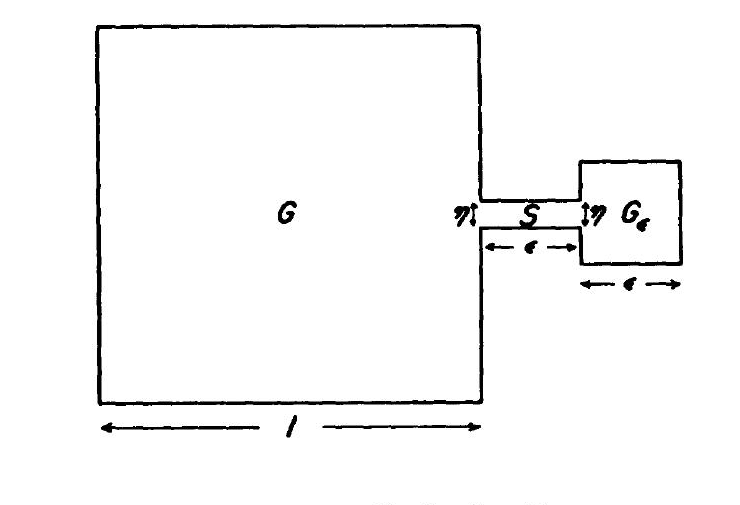
\includegraphics[width=.56\linewidth]{figures/ch06_domain_counterexample.png}\par}\smallskip

For, consider a function $\varphi$ in $G'$ which is equal to $-1/\epsilon$ in $G_\epsilon$, and to a constant $c$ in $G$, and which falls off linearly in $S$ from $c$ to $-1/\epsilon$. Let the constant $c$ be chosen in such a way that the integral of $\varphi$ over $G'$ vanishes. If $\epsilon$ is sufficiently small, $c$ is arbitrarily close to $0$. The integral $\mathfrak D[\varphi]$ over $G'$ will be of the order $\eta/\epsilon^3$. If, for example, we choose $\eta=\epsilon^4$, this integral is arbitrarily small while the integral of $\varphi^2$ over $G'$ is arbitrarily close to $1$. Hence, as a consequence of the classical minimal property of the eigenvalues and eigenfunctions, the second eigenvalue of $G'$ is certainly arbitrarily small. If we permit $\epsilon$ to approach zero, the second eigenvalue of $G'$ will certainly converge to zero if $\eta/\epsilon^3$ does. But the second eigenvalue of $G$ is positive; hence it is not the limit of the second eigenvalue of $G'$ although the boundary of $G'$ converges to the boundary of $G$.}

Approximation of the domain $G$ by the domain $G'$ in the stronger sense is defined analytically in the following way:

Let $G$ together with its boundary be transformed pointwise into the domain $G'$ together with its boundary by equations of the form
\begin{equation}\tag{21}
x'=x+g(x,y),\qquad y'=y+h(x,y);
\end{equation}
here the functions $g,h$ are continuous and have piecewise continuous first derivatives throughout the domain, and both $g,h$ and their first derivatives are less in absolute value than a small positive number $\epsilon$. Then we say that \emph{the domain $G$ is approximated by the domain $G'$ with the degree of accuracy $\epsilon$.}

When $\epsilon$ approaches zero we say that $G'$ is deformed continuously into $G$. We shall prove the following theorem:

\textsc{Theorem 10:} \emph{For any of the boundary conditions considered, the $n$-th eigenvalue of the differential equation $L[u]+\lambda\rho u=0$ varies continuously when the domain $G$ is deformed continuously in the sense defined above.}

Proof: Consider a sequence of domains $G'$ for which the above numbers $\epsilon$ converge to zero. We solve equations (21) for $x$ and $y$, set $\varphi(x,y)=\varphi'(x',y')$, $p(x,y)=p'(x',y')$ etc., $\sigma(x(s),y(s))=\tau(s)$, and transform the two integrals which constitute $\mathfrak D[\varphi]$ into an integral over the domain $G'$ and one over its boundary $\Gamma'$.

In this way we obtain an eigenvalue variational problem for the domain $G$, with coefficients differing arbitrarily little from the original coefficients. Accordingly, continuous dependence may be proved by methods analogous to those which led to Theorems 8 and 9. We shall carry out the proof in detail:

The integral $D[\varphi]$ is transformed into the integral
\begin{equation}\tag{22}
\iint_{G'}\Bigl\{p'\Bigl[\bigl(\varphi_{x'}'(1+g_x)+\varphi_{y'}'h_x\bigr)^2
+\bigl(\varphi_{x'}'g_y+\varphi_{y'}'(1+h_y)\bigr)^2\Bigr]
+q'\varphi'^2\Bigr\}M^{-1}\,dx'\,dy',
\end{equation}
where $M$ stands for the functional determinant
\[
M=\left(1+\frac{\partial g}{\partial x}\right)\left(1+\frac{\partial h}{\partial y}\right)
-\frac{\partial g}{\partial y}\frac{\partial h}{\partial x}
\]
which is arbitrarily close to $1$ if $\epsilon$ is sufficiently small. The integral over the boundary becomes
\[
\int_\Gamma p\sigma\varphi^2\,ds
=\int_{\Gamma'}p'\tau(s)\varphi'^2\frac{ds}{ds'}\,ds',
\]
where $ds'$ denotes the element of arc on the boundary $\Gamma'$ of $G'$.

If in general we define
\[
D'[\psi]=\iint_{G'}\{p(\psi_x^2+\psi_y^2)+q\psi^2\}\,dx\,dy,
\qquad
\mathfrak D'[\psi]=D'[\psi]+\int_{\Gamma'}p\tau(s)\psi^2\,ds',
\]
then the integrand in (22) differs from the integrand of $D'[\varphi']$ by the factors $M^{-1}$ and $p/p'$ (which differ arbitrarily little from $1$) and by the additive terms in which $\varphi_{x'}'^2$, $\varphi_{y'}'^2$, $\varphi_{x'}'\varphi_{y'}'$, and $\varphi'^2$, multiplied by factors which converge to zero with $\epsilon$, appear. Using the inequality
\[
2\left|\iint_{G'}\varphi_{x'}'\varphi_{y'}'\,dx'\,dy'\right|
\le\iint_{G'}(\varphi_{x'}'^2+\varphi_{y'}'^2)\,dx'\,dy',
\]
we obtain the relation
\[
D[\varphi]=(1+\delta)D'[\varphi'],
\]
where $\delta$ denotes a quantity which approaches zero with $\epsilon$. This notation will be used in the sequel, although $\delta$ will not always stand for the same quantity. Since $ds/ds'$ is arbitrarily close to $1$, for sufficiently small $\epsilon$, we have
\[
\int_{\Gamma'}p'\tau(s)\varphi'^2\frac{ds}{ds'}\,ds'
=(1+\delta)\int_{\Gamma'}p\tau(s)\varphi'^2\,ds'
\]
and therefore
\[
\mathfrak D[\varphi]=(1+\delta)\mathfrak D'[\varphi'].
\]

Furthermore, we must transform the auxiliary conditions (3a) and (17) imposed on the functions $\varphi$ in \S1. Thus we obtain the expressions
\[
\iint_G\rho\varphi^2\,dx\,dy
=\iint_{G'}\rho'M^{-1}\varphi'^2\,dx'\,dy'=1,
\]
\[
\iint_G\rho\varphi v_i\,dx\,dy
=\iint_{G'}\rho'M^{-1}\varphi'v_i'\,dx'\,dy'=0
\qquad(i=1,2,\ldots,n-1).
\]
We multiply the function $\varphi'$ by a constant factor and the functions $v_i'$ by $M^{-1}\rho'/\rho$; these factors all differ arbitrarily little from $1$ for small $\epsilon$. The resulting functions $\varphi''$ and $v_i''$ satisfy the relations
\[
\iint_{G'}\rho\varphi''^2\,dx'\,dy'=1,
\]
\[
\iint_{G'}\rho\varphi''v_i''\,dx'\,dy'=0
\qquad(i=1,2,\ldots,n-1).
\]
We find that
\[
\mathfrak D[\varphi]=(1+\delta)\mathfrak D'[\varphi'']
\]
holds and that the function $\varphi''$ satisfies the conditions of the maximum-minimum problem which characterizes the $n$-th eigenvalue for $G'$; here the functions $v_i''$ in $G'$ correspond to the functions $v_i$ in $G$. The domain of variability of the functions $v_i''$ is just the set of admitted functions over $G'$; it follows that the maximum-minimum of the left side can differ from that of the right only by a factor which approaches $1$ as $\epsilon$ approaches zero, which proves Theorem 10. The above reasoning results in the following sharper form of this theorem:

\textsc{Corollary to Theorem 10:} \emph{If a domain $G$ is deformed into a domain $G'$ by the transformation (21) in such a way that}
\[
\left|\frac{\partial g}{\partial x}\right|<\epsilon,
\quad\left|\frac{\partial g}{\partial y}\right|<\epsilon,
\quad\left|\frac{\partial h}{\partial x}\right|<\epsilon,
\quad\left|\frac{\partial h}{\partial y}\right|<\epsilon,
\]
\emph{where $\epsilon$ is any small positive number, then there exists a number $\eta$, depending only on $\epsilon$ and approaching zero with $\epsilon$, such that for every $n$ and for any one of the boundary conditions in question the $n$-th eigenvalues $\mu_n$, $\mu_n'$ for the domains $G$ and $G'$, respectively, satisfy the relation}
\[
\left|\frac{\mu_n'}{\mu_n}-1\right|<\eta.
\]

For the boundary condition $u=0$, in which no normal derivatives appear, the theorem on continuous dependence holds under less restrictive conditions:

\textsc{Theorem 11:} \emph{For the boundary condition $u=0$, the $n$-th eigenvalue of the equation $L[u]+\lambda\rho u=0$ is a continuous function of the domain $G$, even though the normals are no longer required to vary continuously when the domain is continuously deformed.}

In fact, we can always enclose the boundaries of any two domains $G$ and $G'$, which are sufficiently close together (but for which the normals at neighboring boundary points do not necessarily have neighboring directions), between the boundaries of two domains $B$ and $B'$ which are sufficiently close in the more restrictive sense. Since by Theorem 3 the $n$-th eigenvalue for the boundary condition $u=0$ is a monotonic function of the domain, the $n$-th eigenvalues of $G$ and $G'$ must lie between those of $B$ and $B'$, which by Theorem 10 are themselves close together. This proves Theorem 11.

If we do not pass to the limit $\epsilon\to0$, the preceding considerations furnish the following more general result:

\emph{If two domains $G$ and $G'$ are related to each other by a point transformation of the above type such that the absolute value of the functional determinant is uniformly bounded, and if $\lambda_n$ and $\lambda_n'$ denote the $n$-th eigenvalues of the domains $G$ and $G'$, respectively, then for sufficiently large $n$ the quotient $\lambda_n/\lambda_n'$ lies between positive bounds which are independent of $n$.}

\section{Completeness and Expansion Theorems}
\subsection{Completeness of the Eigenfunctions}
In connection with the variational problems for the quotients $\mathfrak D[\varphi]/H[\varphi]$ considered in \S\S1 and 2, we obtained the relation
\[
\lim_{n\to\infty}\lambda_n=\infty.
\]
For the result it was essential that $H[\varphi]$ be positive definite, i.e. that $H[\varphi]$ can assume only non-negative values and vanishes only if the integrand $\varphi$ vanishes. Using the above limit relation we shall now prove the completeness theorem in a sharper form.

\emph{The system of eigenfunctions associated with the quotient $\mathfrak D[\varphi]/H[\varphi]$ is complete in the following sense: For any continuous function $f$ and any positive $\epsilon$, arbitrarily small, we can find a finite linear combination}
\[
\alpha_1u_1+\alpha_2u_2+\cdots+\alpha_nu_n=\omega_n
\]
\emph{of the eigenfunctions such that}
\[
H[f-\omega_n]<\epsilon.
\]
\emph{We obtain the best approximation, i.e. the smallest value of $H[f-\omega_n]$, with the Fourier coefficients}
\[
\alpha_i=c_i=H[f,u_i].
\]
\emph{These satisfy the completeness relation}
\begin{equation}\tag{23}
H[f]=\sum_{i=1}^\infty c_i^2.
\end{equation}

Here, as in the case of arbitrary orthogonal functions, it follows from relations (8) of \S1 that the best mean approximation of $f$ with respect to $H$ by a linear combination of the first $n$ eigenfunctions, that is, the smallest value of $H[f-\omega_n]$, is attained when $\alpha_i=c_i=H[f,u_i]$ (the coefficients are independent of $n$). The relation
\[
0\le H\left[f-\sum_{i=1}^n c_i u_i\right]=H[f]-\sum_{i=1}^n c_i^2
\]
immediately implies the convergence of the infinite series $\sum_{i=1}^\infty c_i^2$ or, more precisely, the Bessel inequality $\sum_{i=1}^\infty c_i^2\le H[f]$.

To prove not only this inequality but the completeness relation (23), we assume first that the function $f$ satisfies the admissibility conditions of the variational problem. Then the function
\[
\rho_n=f-\sum_{i=1}^n c_i u_i
\]
satisfies the orthogonality relations
\begin{equation}\tag{24}
H[\rho_n,u_i]=0\qquad(i=1,2,\ldots,n)
\end{equation}
and, by \S1 equation (7), also the orthogonality relations
\begin{equation}\tag{24'}
\mathfrak D[\rho_n,u_i]=0\qquad(i=1,2,\ldots,n).
\end{equation}
From (24) and from the minimal property of $\lambda_{n+1}$, we find
\begin{equation}\tag{25}
\lambda_{n+1}H[\rho_n]\le\mathfrak D[\rho_n].
\end{equation}
On the other hand, $\mathfrak D[\rho_n]$ is bounded, since
\[
\mathfrak D[f]=\mathfrak D\left[\sum_{i=1}^n c_i u_i\right]
+2\mathfrak D\left[\sum_{i=1}^n c_i u_i,\rho_n\right]
+\mathfrak D[\rho_n];
\]
therefore, from relations (24') we have
\[
\mathfrak D[f]=\mathfrak D\left[\sum_{i=1}^n c_i u_i\right]+\mathfrak D[\rho_n].
\]
$\mathfrak D[\sum_{i=1}^n c_i u_i]$ equals $\sum_{i=1}^n\lambda_i c_i^2$ and remains greater than a fixed bound as $n$ increases since only a finite number of eigenvalues can be negative. Thus $\mathfrak D[\rho_n]$ is bounded from above.

In virtue of relation (25) and the infinite growth of $\lambda_{n+1}$,
\[
H[f]-\sum_{i=1}^n c_i^2=H[\rho_n]\to0\qquad\text{for }n\to\infty,
\]
which proves the completeness relation (23) and therefore the completeness of the eigenfunctions.

If the continuous function $f$ fails to satisfy the admissibility conditions of the problem, we can approximate it by a function $f^*$ which does satisfy these conditions in such a way that $H[f-f^*]<\epsilon/4$, and then approximate $f^*$ by a function $f_n^*=\sum_{i=1}^n c_i^*u_i$ with the property $H[f^*-f_n^*]<\epsilon/4$. Then, since
\[
H[f-f_n^*]=H[f-f^*]+H[f^*-f_n^*]+2H[f-f^*,f^*-f_n^*],
\]
we have from the Schwarz inequality $H[f-f_n^*]<\epsilon$ and from the minimal property of $\rho_n$, $H[\rho_n]<\epsilon$. This proves the completeness theorem for functions which are only continuous.

The completeness of the system of solutions of the variational problem implies that these solutions actually represent the totality of eigenfunctions of the corresponding differential equation problem (cf. the reasoning frequently used in Chapter V, e.g. page 301).

From the completeness relation (23) we easily deduce the more general completeness relation for a pair of functions $f$ and $g$,
\begin{equation}\tag{23a}
H[f,g]=\sum_{i=1}^\infty H[f,u_i]H[g,u_i].
\end{equation}
By a slight addition to our argument, relation (23) can be supplemented by
\begin{equation}\tag{23b}
\mathfrak D[f]=\sum_{i=1}^\infty\lambda_i c_i^2
\end{equation}
provided $\mathfrak D[f]$ is finite.

We assume first that a continuous $L[f]=g$ exists, with $H[g]$ finite. Then using Green's formula, we write
\[
\mathfrak D[f]=-H[f,g].
\]
Applying the completeness relation (23a) to the inner product $H[f,g]$ we obtain
\[
H[f,g]=\sum_{i=1}^\infty H[f,u_i]H[g,u_i].
\]
Green's formula, together with (23a) and $L[u_i]=-\lambda_i u_i$ immediately yields
\[
H[g,u_i]=H[f,L[u_i]]=-\lambda_iH[f,u_i].
\]
Thus (23b) is proved, since $H[f,u_i]=c_i$.

If $L[f]=g$ does not satisfy the above assumption we obtain the result by a suitable approximation of $f$; the method is similar to that used to prove (23).

\subsection{The Expansion Theorem}
In the case of a single independent variable it is not difficult to derive from our result the theorems on the expansion of arbitrary functions in terms of eigenfunctions, thus supplementing the completeness theorem. This can be done under essentially weaker assumptions than those in Chapter V.

We shall prove: \emph{Every function $f(x)$ which satisfies the admissibility conditions of an eigenvalue variational problem may be expanded in an absolutely and uniformly convergent series $\sum_{n=1}^\infty c_nu_n$ in terms of the eigenfunctions.}

Because of the completeness of the orthonormal system $\sqrt\rho\,u_n$, it is sufficient to prove that the series $\sum_{n=1}^\infty c_nu_n$, where $c_n=\int_0^\pi\rho f u_n\,dx$, converges uniformly (cf. Ch. II, p. 54). To prove this, we again consider the function $\rho_n=f-\sum_{\nu=1}^n c_\nu u_\nu$. As above, page 424, we see that
\[
\mathfrak D[\rho_n]=\mathfrak D[f]-\sum_{\nu=1}^n c_\nu^2\lambda_\nu.
\]
For sufficiently large $n$, say $n\ge N$, we have $\lambda_{n+1}\ge0$, and thus $\mathfrak D[\rho_n]\ge0$. Therefore the series $\sum_{\nu=1}^\infty c_\nu^2\lambda_\nu$ converges, since its terms are non-negative for $\nu>N$. Schwarz's inequality yields
\[
\left(\sum_{n=h}^k c_nu_n(x)\right)^2
\le\sum_{n=h}^k c_n^2\lambda_n\sum_{n=h}^k\frac{u_n^2(x)}{\lambda_n}
\le\sum_{n=1}^\infty c_n^2\lambda_n\sum_{n=h}^k\frac{u_n^2(x)}{\lambda_n}.
\]
Now, from Ch. V, \S11, 3 we know that $|u_n(x)|<C$, where $C$ is a constant independent of $n$. Since, by \S2, 2 and 3, $\lambda_n/n^2$ lies between positive bounds, and since $\sum_{n=1}^\infty1/n^2$ converges, $\sum_{n=h}^k u_n^2(x)/\lambda_n$ is arbitrarily small uniformly in $x$ for sufficiently large $h$ and $k$, and thus the same is true of $|\sum_{n=h}^k c_nu_n(x)|$. This means that the above series converges absolutely and uniformly, which completes the proof of the expansion theorem.

Our considerations and results remain valid even when singularities occur, as in the case of Legendre and Bessel eigenfunctions. However, our proof of the expansion theorem then holds only if we exclude from the domain an arbitrarily small neighborhood of the singular points, since boundedness of the normalized eigenfunctions has not been proved for such a neighborhood.

\subsection{Generalization of the Expansion Theorem}
The asymptotic expressions for the Sturm--Liouville eigenfunctions (Ch. V, \S11, 5) permit us to generalize the expansion theorem just proved. In fact, we can prove the theorem: \emph{every piecewise continuous function defined in the fundamental domain with a square-integrable\footnote{We say that the derivative is square-integrable if the integral of the square of the derivative is bounded for all the intervals of the fundamental domain in which the function is continuous.} first derivative may be expanded in an eigenfunction series which converges absolutely and uniformly in all subdomains free of points of discontinuity; at the points of discontinuity it represents (like the Fourier series) the arithmetic mean of the right- and left-hand limits.} (It should be remarked that this theorem does \emph{not} require that the functions to be expanded satisfy the boundary conditions.)

As in \S2, 3, we suppose the differential equation to be written in the form (18),
\[
z''-rz+\lambda z=0,
\]
for the function $z(t)$ in the interval $0\le t\le l$. Then we consider the series
\[
G(t,\tau)=\sum_{n=1}^\infty\frac{z_n(t)z_n(\tau)}{\lambda_n}
\]
in which $z_n$ denotes the $n$-th eigenfunction of the above differential equation, say for the boundary condition $z=0$.

Application of the asymptotic formulas (70) and (71) of Chapter V, together with formula (19), yields
\[
G(t,\tau)=\frac{2}{\pi}\sum_{n=1}^\infty
\frac{\sin\frac{n\pi}{l}t\cos\frac{n\pi}{l}\tau}{n}
+\sum_{n=1}^\infty\psi_n(t,\tau),
\]
where $\psi_n(t,\tau)=O(1/n^2)$, so that $G(t,\tau)$ differs only by an absolutely and uniformly convergent series from
\[
G^*(t,\tau)=\frac{2}{\pi}\sum_{n=1}^\infty
\frac{\sin\frac{n\pi}{l}t\cos\frac{n\pi}{l}\tau}{n}
=\frac1\pi\sum_{n=1}^\infty\frac1n\left(
\sin\frac{n\pi}{l}(t+\tau)+\sin\frac{n\pi}{l}(t-\tau)\right).
\]
As we saw in Ch. II, \S5, 1, this series has the following properties: For fixed $\tau$ $(0<\tau\le l)$ it converges absolutely and uniformly for all $t$ of a closed interval which satisfy the conditions $|t+\tau|>\epsilon$, $|t-\tau|>\epsilon$ for $\epsilon>0$. Since $\tau>0$ and $t>0$, this means that the interval cannot contain the point $t=\tau$. Therefore, although for $t\ne\tau$ the series represents a continuous function, its sum has a finite jump at $t=\tau$ and at this point, again by Ch. II, \S5, it is equal to the arithmetic mean of the right- and left-hand limits.

In the case of an arbitrary function which satisfies the above conditions, we remove the discontinuities by adding a suitable sum
\[
\sum_i a_iG(t,\tau_i)
\]
which is chosen (if necessary) in such a way that the boundary condition is satisfied. We obtain a function satisfying the conditions of the general expansion theorem already proved in subsection 2; this function may, therefore, be expanded in an absolutely and uniformly convergent eigenfunction series. However, as we have just seen, the additional sum may itself be represented by an eigenfunction series with the properties stated in the generalized expansion theorem (see page 427); thus we have proved this theorem for the expansion in terms of the eigenfunctions of the differential equation (18). If we transform the variables $z,t$ back to $y,x$ and the differential equation to the general Sturm--Liouville form, we immediately obtain the expansion theorem for the eigenfunctions $y_n(x)$ of the original differential equation; for, except for constant factors, these eigenfunctions are obtained by multiplying the eigenfunctions $z_n$ by the same nowhere-vanishing function.

\section{Asymptotic Distribution of Eigenvalues}
The method of \S2, 2 and \S2, 3 for one independent variable can also be used in the study of the asymptotic behavior of the $n$-th eigenvalue for several independent variables. We obtain a result significant for physical problems: \emph{the asymptotic behavior of the eigenvalues for differential equations with constant coefficients does not depend on the shape but only on the size of the fundamental domain.}

\subsection{The Equation $\Delta u+\lambda u=0$ for a Rectangle}
In the case of a rectangle of sides $a$ and $b$, the eigenfunctions and eigenvalues of $\Delta u+\lambda u=0$ are known explicitly (see Ch. V, \S5, 4). In fact, for the boundary condition $u=0$ they are given---up to a normalizing factor---by the expressions
\[
\sin\frac{l\pi x}{a}\sin\frac{m\pi y}{b},
\qquad
\pi^2\left(\frac{l^2}{a^2}+\frac{m^2}{b^2}\right)
\qquad(l,m=1,2,3,\ldots),
\]
and for the boundary condition $\partial u/\partial n=0$ by the expressions
\[
\cos\frac{l\pi x}{a}\cos\frac{m\pi y}{b},
\qquad
\pi^2\left(\frac{l^2}{a^2}+\frac{m^2}{b^2}\right)
\qquad(l,m=0,1,2,3,\ldots).
\]

If the number of eigenvalues less than a bound $\lambda$ is denoted in the first case by $A(\lambda)$ and in the second case by $B(\lambda)$, then $A(\lambda)$ and $B(\lambda)$ are equal to the number of integral solutions of the inequality
\[
\frac{l^2}{a^2}+\frac{m^2}{b^2}\le \frac{\lambda}{\pi^2};
\]
here $l>0$, $m>0$ for the boundary condition $u=0$ and $l\ge0$, $m\ge0$ for the condition $\partial u/\partial n=0$. Simple \emph{asymptotic expressions} for the desired numbers $A(\lambda)$ and $B(\lambda)$ may now be derived for large $\lambda$. $B(\lambda)$, for example, is precisely equal to the number of lattice points with integral coordinates in the sector of the ellipse
\[
\frac{x^2}{a^2}+\frac{y^2}{b^2}=\frac{\lambda}{\pi^2}
\]
which lies in the quadrant $x\ge0$, $y\ge0$. For sufficiently large $\lambda$ the ratio of the area of this sector to the number of lattice points contained in it is arbitrarily close to 1. If a unit square lying above and to the right of each lattice point is associated with it, then the region formed by these squares contains this sector of the ellipse; however, if we omit the squares through which the ellipse passes,--let the number of these be $R(\lambda)$--then the region which remains is contained entirely within this sector of the ellipse. We therefore have between the areas the inequality
\[
B(\lambda)-R(\lambda)\le \lambda\frac{ab}{4\pi}\le B(\lambda).
\]
The arc of the ellipse contained in two adjoining boundary squares has, for sufficiently large $\lambda$, at least the length 1. Hence $R(\lambda)-1$ is at most equal to twice the arc length of the quarter ellipse, and this increases only with $\sqrt\lambda$. We thus obtain the asymptotic formula
\[
\lim_{\lambda\to\infty}\frac{B(\lambda)}{\lambda}=\frac{ab}{4\pi}
\]
or
\[
B(\lambda)\sim\lambda\frac{ab}{4\pi}.
\]
More precisely, we can write
\[
B(\lambda)=\frac{ab}{4\pi}\lambda+\theta c\sqrt\lambda,
\]
where $c$ is a constant independent of $\lambda$, and $|\theta|<1$. This formula is valid for both boundary conditions considered; i.e., it also holds for $A(\lambda)$, since the number of lattice points lying on the line-segments in the boundary of the sector of the ellipse is asymptotically equal to $(a+b)\sqrt\lambda/\pi$. If the eigenvalues are written in a sequence $\lambda_1,\lambda_2,\ldots$ ordered according to magnitude, we can calculate the $n$-th eigenvalue asymptotically by setting $A(\lambda_n)=n$ and $B(\lambda_n)=n$. We obtain
\[
\lambda_n\sim\frac{4\pi}{ab}A(\lambda_n)\sim\frac{4\pi}{ab}n
\]
or
\[
\lim_{n\to\infty}\frac{\lambda_n}{n}=\frac{4\pi}{ab}.
\]

\subsection{The Equation $\Delta u+\lambda u=0$ for Domains Consisting of a Finite Number of Squares or Cubes}
Now we consider the equation $\Delta u+\lambda u=0$ for a domain $G$ which may be decomposed into a finite number, say $h$, of squares $Q_1,Q_2,\ldots,Q_h$ (or cubes in the case of three independent variables) of side $a$. Such domains will be called square-domains (or cube-domains). The area of $G$ is then $f=ha^2$ (or its volume is $V=ha^3$).

As before $\theta$ will denote a number between $-1$ and $+1$, and $c$ or $C$ a positive constant. When no misunderstanding seems likely we shall denote different values of $\theta$ and $c$ or $C$ by the same symbol without explicitly distinguishing between them by means of indices.

For a domain $G$ consisting of $h$ squares, let $A(\lambda)$ be the number of eigenvalues less than a bound $\lambda$ for the boundary condition $u=0$ and let $B(\lambda)$ be the corresponding number for the boundary condition $\partial u/\partial n=0$. Denoting by $A_{Q_1}(\lambda),A_{Q_2}(\lambda),\ldots,A_{Q_h}(\lambda)$ the corresponding numbers for the subsquares with the boundary conditions $u=0$, and by $B_{Q_1}(\lambda),B_{Q_2}(\lambda),\ldots,B_{Q_h}(\lambda)$ these numbers with the boundary conditions $\partial u/\partial n=0$, we have from subsection 1
\begin{equation}\tag{26}
A_{Q_i}(\lambda)=\frac{a^2}{4\pi}\lambda+\theta ca\sqrt\lambda,
\qquad
B_{Q_i}(\lambda)=\frac{a^2}{4\pi}\lambda+\theta'ca\sqrt\lambda
\qquad(i=1,2,\ldots,h).
\end{equation}
Combining Theorem 5 with Theorems 2 and 4 (see \S2) we have
\[
A_{Q_1}(\lambda)+\cdots+A_{Q_h}(\lambda)\le A(\lambda)
\le B_{Q_1}(\lambda)+\cdots+B_{Q_h}(\lambda).
\]
Since the numbers $A_{Q_i}(\lambda),B_{Q_i}(\lambda)$ have the form given by equations (26), we conclude
\[
A(\lambda)=\frac{f}{4\pi}\lambda+\theta ca\sqrt\lambda.
\]
In other words, the following theorem holds:

\textsc{Theorem 12:} \emph{For all boundary conditions considered, the number $A(\lambda)$ of eigenvalues less than a bound $\lambda$ of the differential equation $\Delta u+\lambda u=0$ for a square-domain of area $f$ is asymptotically equal to $f\lambda/4\pi$; that is,}
\begin{equation}\tag{27}
\lim_{\lambda\to\infty}\frac{A(\lambda)}{f\lambda}=\frac1{4\pi}.
\end{equation}
\emph{More precisely, for all sufficiently large $\lambda$ the relation}
\begin{equation}\tag{28}
\left|\frac{4\pi A(\lambda)}{f\lambda}-1\right|<\frac{C}{\sqrt\lambda}
\end{equation}
\emph{holds, where $C$ is a constant independent of $\lambda$.}

If $\rho_n$ denotes the $n$-th eigenvalue corresponding to one of the boundary conditions in question, this theorem or relation (28) is equivalent to equation
\begin{equation}\tag{29}
\rho_n=\frac{4\pi}{f}n+\theta c\sqrt n,
\end{equation}
where again $-1\le\theta\le1$ and $c$ is a constant independent of $n$. To see this one has only to set $A(\rho_n)=n$ in (28).

Theorem 12 remains valid even if the function $\sigma$ in the boundary condition $\partial u/\partial n+\sigma u=0$ assumes negative values. This will again be shown with the aid of the remarks of \S2, 5. First we note that according to Theorem 5, the $n$-th eigenvalue $\mu_n$ for the boundary condition $\partial u/\partial n+\sigma u=0$ can surely be no greater than the $n$-th eigenvalue $\lambda_n$ for the boundary condition $u=0$. Thus we may assume from the outset that the expression
\[
\mathfrak D[\varphi]=D[\varphi]+\int_\Gamma p\sigma\varphi^2\,ds,
\]
whose maximum-minimum is clearly $\mu_n$, never exceeds the bound $\lambda_n$ for any of the functions $\varphi$ which are admissible in the variational problem with the boundary condition $u=0$.

Now by \S2, 5 we have
\[
\left|\int_\Gamma p\sigma\varphi^2\,ds\right|<c_1\sqrt{|D[\varphi]|}+c_2,
\]
where $c_1,c_2$ are numerical constants; thus we have
\[
D[\varphi]-c_1\sqrt{|D[\varphi]|}-c_2<\mathfrak D[\varphi]
<D[\varphi]+c_1\sqrt{|D[\varphi]|}+c_2.
\]
From the assumption $\mathfrak D[\varphi]\le\lambda_n$ it follows that
\[
D[\varphi]-c_1\sqrt{|D[\varphi]|}-c_2<\lambda_n,
\]
and this in turn implies that, for increasing $n$, $D[\varphi]$ can increase no faster than $\lambda_n$, or in other words that there must be a relation of the form
\[
D[\varphi]<c_3\lambda_n,
\]
where $c_3$ also denotes a constant. Since relation (29) holds for $\rho_n=\lambda_n$ we have, under the assumptions made with respect to $\varphi$,
\[
D[\varphi]-c_4\sqrt n\le\mathfrak D[\varphi]\le D[\varphi]+c_4\sqrt n;
\]
this relation is valid for the lower bounds of the expressions $\mathfrak D[\varphi]$ for given functions $v_1,v_2,\ldots,v_{n-1}$, and hence also for the maxima of these lower bounds. The maximum-minimum of $D[\varphi]$ is the $n$-th eigenvalue for the boundary condition $\partial u/\partial n=0$, for which relation (29) has already been proved. Therefore (29) follows directly for the maximum of the lower bounds of $\mathfrak D[\varphi]$, i.e. for the $n$-th eigenvalue $\mu_n$ with the boundary condition $\partial u/\partial n+\sigma u=0$; this relation is equivalent to the assertion of Theorem 12.

If there are three independent variables instead of two, the preceding discussion remains unchanged except for the expressions $A_{Q_i}$ and $B_{Q_i}$ for the number of eigenvalues less than the bound $\lambda$ under the boundary conditions $u=0$ and $\partial u/\partial n=0$, respectively. We find, in fact, that
\begin{equation}\tag{26a}
A_{Q_i}(\lambda)=\frac1{6\pi^2}a^3\lambda^{3/2}+\theta ca^2\lambda,
\qquad
B_{Q_i}(\lambda)=\frac1{6\pi^2}a^3\lambda^{3/2}+\theta ca^2\lambda
\end{equation}
holds and obtain

\textsc{Theorem 13:} \emph{Consider the differential equation $\Delta u+\lambda u=0$ for a polyhedron of volume $V$ consisting of a finite number $k$ of congruent cubes. For all boundary conditions in question the number $A(\lambda)$ of eigenvalues less than a bound $\lambda$ is asymptotically equal to $V\lambda^{3/2}/6\pi^2$, i.e.}
\begin{equation}\tag{27a}
\lim_{\lambda\to\infty}\frac{A(\lambda)}{V\lambda^{3/2}}=\frac1{6\pi^2}.
\end{equation}
\emph{More precisely, for sufficiently large $\lambda$ we have the formula}
\begin{equation}\tag{28a}
\left|\frac{6\pi^2A(\lambda)}{V\lambda^{3/2}}-1\right|<C\frac1{\sqrt\lambda},
\end{equation}
\emph{in which $C$ is a constant independent of $\lambda$.}\footnote{It is not in general possible to obtain a sharper estimate of the error in this asymptotic estimate of $A(\lambda)$, since for both the square and the cube the indicated order of magnitude of the error is actually attained.}

\subsection{Extension to the General Differential Equation $L[u]+\lambda\rho u=0$}
We shall now extend Theorem 13 to the general self-adjoint differential equation (1). We assume that, by repeated halving of the length of the edge $a$, the subdivision of the domain $G$ into squares or cubes has been refined in such a way that in the resulting subdomains the difference between the largest and the smallest values of the functions $p$ and $\rho$ is always less than a given small positive number $\epsilon$. \emph{The function $q$ can have no influence at all on the asymptotic distribution of the eigenvalues}, since the expression $\mathfrak D[\varphi]$, and with it its maximum-minimum, changes by an amount which is bounded, namely, by less than $|q_M|/\rho_m$, here $q_M$ and $\rho_m$ have the same meaning as before. Accordingly, we set $q=0$ without affecting the asymptotic distribution.

We consider the case of a plane domain $G$ consisting of a finite number of squares. Let the number of squares again be $h$, and let the lengths of their sides be $a$. $A'(\lambda)$ will denote the number of eigenvalues less than a bound $\lambda$ of the differential equation $L[u]+\lambda\rho u=0$ for the domain $G$; any of the boundary conditions considered may be used, but for the condition $\partial u/\partial n+\sigma u=0$ we must make the restrictive assumption $\sigma\ge0$. We denote the subsquares by $Q_1,Q_2,\ldots,Q_h$, and the associated numbers of eigenvalues of the differential equation less than a bound $\lambda$ by $A'_{Q_1}(\lambda),A'_{Q_2}(\lambda),\ldots,A'_{Q_h}(\lambda)$ for the boundary condition $u=0$, and by $B'_{Q_1}(\lambda),B'_{Q_2}(\lambda),\ldots,B'_{Q_h}(\lambda)$ for the boundary condition $\partial u/\partial n=0$. From Theorems 2, 4 and 5 we obtain
\begin{equation}\tag{30}
A'_{Q_1}(\lambda)+\cdots+A'_{Q_h}(\lambda)\le A'(\lambda)
\le B'_{Q_1}(\lambda)+\cdots+B'_{Q_h}(\lambda).
\end{equation}
Theorem 7 implies
\[
A'_{Q_i}(\lambda)\ge\frac{\rho_m^{(i)}}{p_M^{(i)}}A_{Q_i}(\lambda),
\qquad
B'_{Q_i}(\lambda)\le\frac{\rho_M^{(i)}}{p_m^{(i)}}B_{Q_i}(\lambda),
\]
where by $p_M^{(i)},\rho_M^{(i)}$ we denote the maxima, and by $p_m^{(i)},\rho_m^{(i)}$ the minima, of the respective functions in the square $Q_i$; again (cf. subsection 2) the number of corresponding eigenvalues of the differential equation $\Delta u+\lambda u=0$ is given by equations (26) and denoted by $A_{Q_i}(\lambda)$ or $B_{Q_i}(\lambda)$. For, substituting $p_M^{(i)}$ for $p$ and $\rho_m^{(i)}$ for $\rho$ in differential equation (1), we see by Theorem 7 that each eigenvalue becomes larger (or at least is not diminished), and thus the number of eigenvalues less than a fixed $\lambda$ decreases (or does not increase). On the other hand, differential equation (1) goes over into the differential equation
\[
\Delta u+\lambda\frac{\rho_m^{(i)}}{p_M^{(i)}}u=0,
\]
whose eigenvalues are the eigenvalues of $\Delta u+\lambda u=0$ multiplied by the factor $p_M^{(i)}/\rho_m^{(i)}$. A corresponding argument holds if $p_m^{(i)}$ is substituted for $p$ and $\rho_M^{(i)}$ for $\rho$.

Furthermore, since $\rho$ and $p$ are continuous functions we have
\[
\iint_G\frac{\rho}{p}\,dx\,dy
=a^2\sum_{i=1}^h\frac{\rho_m^{(i)}}{p_M^{(i)}}+\delta
=a^2\sum_{i=1}^h\frac{\rho_M^{(i)}}{p_m^{(i)}}+\delta',
\]
where the numbers $|\delta|,|\delta'|$ may be made arbitrarily small by making the original subdivision into squares sufficiently fine, that is, by taking $a$ sufficiently small. As in subsection 2, we apply (30) and find
\[
A(\lambda)=\frac{\lambda}{4\pi}\iint_G\frac{\rho}{p}\,dx\,dy
+\lambda\delta''+\theta c\sqrt\lambda,
\]
where $|\delta''|$ also is arbitrarily small. This is equivalent to the following statement about the asymptotic distribution of eigenvalues:

\textsc{Theorem 14:} \emph{For the differential equation $L[u]+\lambda\rho u=0$, under any of the boundary conditions considered, the number $A(\lambda)$ of eigenvalues less than a given bound $\lambda$ for a square-domain $G$ is asymptotically equal to}
\[
\frac{\lambda}{4\pi}\iint_G\frac{\rho}{p}\,dx\,dy;
\]
\emph{in other words the relation}
\begin{equation}\tag{31}
\lim_{\lambda\to\infty}\frac{A(\lambda)}{\lambda}
=\frac1{4\pi}\iint_G\frac{\rho}{p}\,dx\,dy
\end{equation}
\emph{holds.}

As in subsection 2, we see that the original assumption $\sigma\ge0$ is unnecessary.

Analogous considerations for three-dimensional space lead to

\textsc{Theorem 15:} \emph{For the differential equation $L[u]+\lambda\rho u=0$, under any of the boundary conditions considered, the number of eigenvalues less than a given bound $\lambda$ for a cube-domain $G$ is asymptotically equal to}
\[
\frac1{6\pi^2}\lambda^{3/2}\iiint_G\left(\frac{\rho}{p}\right)^{3/2}\,dx\,dy\,dz;
\]
\emph{in other words, the relation}
\begin{equation}\tag{32}
\lim_{\lambda\to\infty}\frac{A(\lambda)}{\lambda^{3/2}}
=\frac1{6\pi^2}\iiint_G\left(\frac{\rho}{p}\right)^{3/2}\,dx\,dy\,dz
\end{equation}
\emph{holds.}

Finally, we mention that the arguments of the two preceding subsections may be applied also to a \emph{more general domain} consisting of a finite number of rectangles or rectangular parallelepipeds.

\subsection{Asymptotic Distribution of Eigenvalues for an Arbitrary Domain}
With the boundary condition $u=0$, the same asymptotic formulas can easily be proved for an arbitrary domain $G$ which can be approximated from within and without by special regions consisting only of a finite number of squares and differing arbitrarily little in area.

However, we shall aim to establish at once the asymptotic laws for arbitrary $G$ and all the boundary conditions under consideration; for this purpose a somewhat deeper analysis is required.

First we consider a plane domain $G$ whose boundary has continuous curvature and restrict ourselves to the differential equation $\Delta u+\lambda u=0$.

We examine briefly the eigenvalues associated with this differential equation under the boundary condition $\partial u/\partial n=0$, investigating the number of eigenvalues less than a given bound for a few simple domains.

Let $G$ be an isosceles right triangle with sides of length $a$. Every eigenfunction for the triangle is also an eigenfunction for the square which is obtained by reflection across the hypotenuse under the same boundary condition $\partial u/\partial n=0$. For, it is immediately clear that any eigenfunction may be continued into the reflected triangle if the functional value of each original point is assigned to its reflection; in this way the boundary condition $\partial u/\partial n=0$ is satisfied along the entire boundary of the square. The $n$-th eigenvalue for the triangle is therefore also an eigenvalue for the square; hence the $n$-th eigenvalue for the square is certainly no larger than that for the triangle. In other words, \emph{for the triangle, with the boundary condition $\partial u/\partial n=0$, the number of eigenvalues less than a given bound is at most equal to the corresponding number for the square}, that is, the number given by formula (26).

Next, let $G$ be an arbitrary right triangle of sides $a$ and $b$, where we assume $b\le a$. Let side $a$ lie on the $x$-axis, side $b$ on the $y$-axis. By means of the transformation $\xi=x$, $\eta=ay/b$ we transform the triangle $G$ into an isosceles right triangle $G'$ with sides equal to $a$. The expression $D[\varphi]$ then becomes
\[
D[\varphi]=\iint_{G'}\left[\left(\frac{\partial\varphi}{\partial\xi}\right)^2
+\frac{a^2}{b^2}\left(\frac{\partial\varphi}{\partial\eta}\right)^2\right]\frac ba\,d\xi\,d\eta
\]
and the auxiliary condition $H[\varphi]=1$ becomes
\[
\iint_{G'}\varphi^2\frac ba\,d\xi\,d\eta=1,
\]
while the additional auxiliary conditions $H[\varphi,v_i]=0$ of \S1, 4 retain their form under this transformation. Thus, if we omit the insignificant constant factor $b/a$ occurring in both integrals, we can characterize the $n$-th eigenvalue $\kappa_n$ for the triangle as the maximum-minimum of the integral
\[
\iint_{G'}\left[\left(\frac{\partial\varphi}{\partial\xi}\right)^2
+\frac{a^2}{b^2}\left(\frac{\partial\varphi}{\partial\eta}\right)^2\right]d\xi\,d\eta
\]
taken over $G'$, where the maximum-minimum is to be understood in the usual sense. Since $a/b\ge1$, the relation
\[
\iint_{G'}\left[\left(\frac{\partial\varphi}{\partial\xi}\right)^2
+\frac{a^2}{b^2}\left(\frac{\partial\varphi}{\partial\eta}\right)^2\right]d\xi\,d\eta
\ge\iint_{G'}\left[\left(\frac{\partial\varphi}{\partial\xi}\right)^2
+\left(\frac{\partial\varphi}{\partial\eta}\right)^2\right]d\xi\,d\eta
\]
holds, and the maximum-minimum of the left side is therefore at least as large as that of the right side, i.e. it is at least as large as the $n$-th eigenvalue for the isosceles right triangle $G'$, and thus a fortiori larger than the $n$-th eigenvalue of a square of side $a$. Therefore, \emph{under the boundary condition $\partial u/\partial n=0$, the number of eigenvalues less than a given bound for a right triangle with sides not larger than $a$ is certainly no larger than the corresponding number of eigenvalues for the square of side $a$; hence it is no larger than the corresponding number for any larger square.}

Similarly, \emph{the number of eigenvalues less than a given bound for an arbitrary rectangle is never larger than the corresponding number for a square whose side is at least equal to the larger side of the rectangle.}

These results, together with Theorem 4, show that it is possible to obtain an upper bound for the number of eigenvalues less than a given bound whenever the domain in question is composed of a finite number of rectangles and right triangles.

\begin{center}
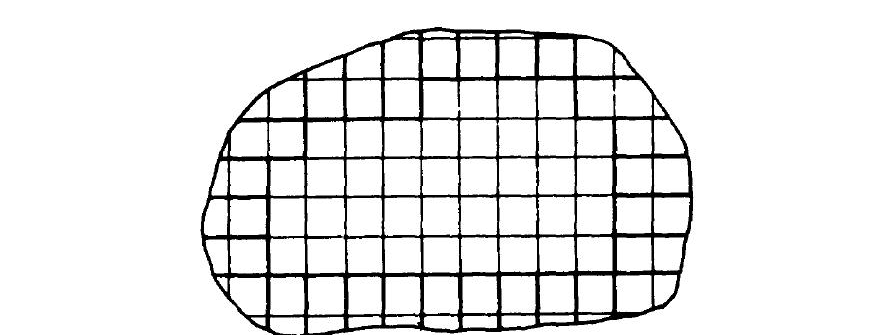
\includegraphics[width=.62\textwidth]{figures/ch06_fig4.png}\\[-0.3em]
{\small Figure 4}
\end{center}

We now consider how the distribution of the eigenvalues is affected by the boundary strip which remains when we approximate the domain $G$ by means of squares. First we define the boundary strip: Let the subdivision into squares be so fine that, for every segment of the boundary of $G$ which is contained in one of the squares, the direction of the normal varies by less than a given small angle $\eta$, whose size will be determined later. (This can be accomplished by repeated halving of the side of the square.) Then, as in Figure 4, we can associate with the boundary $\Gamma$ a number $r$ of adjacent elementary domains $E_1,E_2,\ldots,E_r$ in the following manner: Each domain $E_i$ is bounded either by two perpendicular line-segments $AB,AC$ of the partition, whose lengths lie between $a$ and $3a$, and a segment $BC$ of the boundary (Figure 5), or by a line-segment $AB$ of the partition, two line-segments $AC,BD$ of lengths between $a$ and $3a$ perpendicular to $AB$, and a segment $CD$ of the boundary (Figure 6). We construct a boundary strip $S$ consisting of $r$ domains of this kind, such that when this strip is removed from $G$ a square-domain is left, consisting of $h$ squares $Q_1,Q_2,\ldots,Q_h$.\footnote{We leave it to the reader to carry out this construction: Divide the boundary curve into a finite number of arcs which are of three kinds. On arcs of the first kind the tangents should form an angle of at most $30^\circ$ with the $x$-axis, on those of the second kind one of at most $30^\circ$ with the $y$-axis; on arcs of the third kind the tangents should not form angles with either axis of less than $20^\circ$. The end points of arcs of the first and second kind should have rational abscissae and ordinates, respectively. If the subdivision into squares (on whose sides these end points lie) is sufficiently fine the construction is possible.} The number $r$ is evidently smaller than a constant $C/a$, where $C$ is independent of $a$ and depends essentially on the length of the boundary.

In order to obtain an upper bound for the number $B_{E_i}(\lambda)$ of eigenvalues less than some bound $\lambda$ of the differential equation $\Delta u+\lambda u=0$ for the domain $E_i$ with boundary condition $\partial u/\partial n=0$, we must again try to find a lower bound for the $n$-th eigenvalues. To this end, we take any point on the curvilinear boundary segment of $E_i$ and draw the tangent through it. This tangent together with the straight boundary segments of $E_i$ forms a domain of the type $AB'C'$ (Fig. 5),

\begin{center}
\begin{minipage}{.44\textwidth}\centering
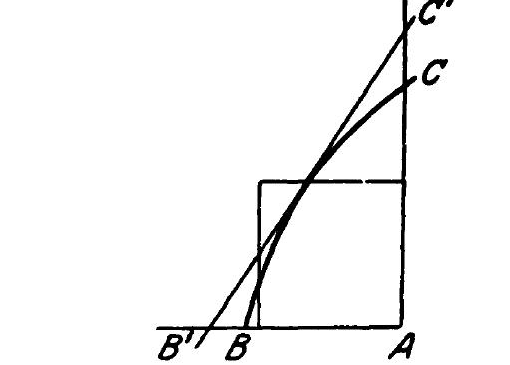
\includegraphics[width=.82\linewidth]{figures/ch06_fig5.png}\\[-0.3em]
{\small Figure 5}
\end{minipage}\hfill
\begin{minipage}{.44\textwidth}\centering
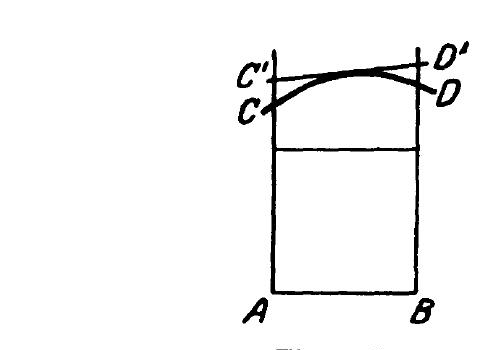
\includegraphics[width=.80\linewidth]{figures/ch06_fig6.png}\\[-0.3em]
{\small Figure 6}
\end{minipage}
\end{center}

e.g. if $\eta$ is sufficiently small it forms a right triangle with sides smaller than $4a$, or else a trapezoid of the type $ABC'D'$ (Figure 6) the sides $AC',BD'$ of which are also smaller than $4a$; the shape of the resulting domain depends on the type to which $E_i$ belongs. We shall denote the domains $AB'C'$ and $ABC'D'$ by $E_i'$. The domain $E_i$ can always be deformed into the domain $E_i'$ by a transformation of the form (21), as discussed in \S2. In the case of domains of the first type, let $A$ be the pole of a system of polar coordinates $\rho,\theta$, and let $\rho=f(\theta)$ be the equation of the curved segment $BC$, $\rho=g(\theta)$ the equation of the line $B'C'$. Then the equations
\[
\theta'=\theta,\qquad \rho'=\rho\frac{g(\theta)}{f(\theta)}
\]
represent a transformation of the curvilinear triangle $E_i$ into the rectilinear triangle $E_i'$. For a domain of the second type $ABCD$, let $AB$ lie along the $x$-axis, let $y=g(x)$ be the equation of the line-segment $C'D'$ and let $y=f(x)$ be the equation of the curved segment $CD$. We then consider the transformation
\[
x'=x,\qquad y'=y\frac{g(x)}{f(x)}.
\]
If we assume that the fundamental interval $a$ is sufficiently small, and therefore that the total rotation of the tangent on the curved segment $CB$ or $CD$ is taken sufficiently small, then the transformations considered here evidently have precisely the form (21), and the quantity denoted by $\epsilon$ in (21) is arbitrarily small. It follows from the corollary to Theorem 10 that the corresponding $n$-th eigenvalues for the domains $E_i$ and $E_i'$ differ only by a factor which itself differs by a small amount from 1, uniformly for all $n$. Hence the same is true also for the corresponding numbers $B_{E_i}(\lambda)$ and $B_{E_i'}(\lambda)$ of eigenvalues less than the bound $\lambda$ for the boundary condition $\partial u/\partial n=0$.

The domain $E_i'$ is either a right triangle with sides smaller than $4a$ or a combination of such a triangle and a rectangle with sides smaller than $3a$; it follows that if $a$ is taken sufficiently small, the number $B_{E_i}(\lambda)$ from some $\lambda$ on satisfies the inequality
\begin{equation}\tag{33}
B_{E_i}(\lambda)<c_1a^2\lambda+c_2a\sqrt\lambda
\end{equation}
where $c_1,c_2$ are numerical constants, to be chosen suitably.

We can now deduce the laws that govern the asymptotic distribution of eigenvalues for the domain $G$. Let $A(\lambda)$, for any of the boundary conditions considered, again denote the number of eigenvalues less than a bound $\lambda$ of the differential equation $\Delta u+\lambda u=0$ for the domain $G$, where again, if necessary, we make the assumption $\sigma\ge0$. Suppose the plane is partitioned into squares of side $a$, inducing a decomposition of the domain $G$ into $h$ squares $Q_1,Q_2,\ldots,Q_h$ and $r$ boundary domains $E_1,E_2,\ldots,E_r$. For the square $Q_i$ the number of eigenvalues less than $\lambda$ is again denoted by $A_i(\lambda)$ for the boundary condition $u=0$ and by $B_i(\lambda)$ for the condition $\partial u/\partial n=0$. The corresponding numbers for the domains $E_i$ are denoted by $A_{E_i}(\lambda)$ and $B_{E_i}(\lambda)$, respectively (we shall use only the numbers $B_{E_i}(\lambda)$).

From equations (26) we have
\[
A_i(\lambda)=\frac{a^2}{4\pi}\lambda+a\theta_1c_1\sqrt\lambda,
\qquad
B_i(\lambda)=\frac{a^2}{4\pi}\lambda+a\theta_2c_2\sqrt\lambda
\]
and, by (33),
\[
B_{E_i}(\lambda)=\theta_3(c_3\lambda a^2+ac_4\sqrt\lambda),
\]
where, as always, $\theta_1,\theta_2,\theta_3$ denote numbers between $-1$ and $+1$, and $c_1,c_2,c_3,c_4$ are constants independent of $a,i$, and $\lambda$.

From Theorems 5, 2, and 4 we find
\[
A_1(\lambda)+A_2(\lambda)+\cdots+A_h(\lambda)\le A(\lambda)
\]
\[
\le B_1(\lambda)+\cdots+B_h(\lambda)+B_{E_1}(\lambda)+\cdots+B_{E_r}(\lambda);
\]
furthermore, we have
\[
A_1(\lambda)+\cdots+A_h(\lambda)
=\frac{ha^2}{4\pi}\lambda+\theta_1c_1ha\sqrt\lambda
=\lambda\left(\frac{ha^2}{4\pi}+\frac{\theta_1c_1ha}{\sqrt\lambda}\right),
\]
\begin{align*}
&B_1(\lambda)+\cdots+B_h(\lambda)+B_{E_1}(\lambda)+\cdots+B_{E_r}(\lambda)\\
&\qquad=\frac{ha^2}{4\pi}\lambda+\theta_2c_2ha\sqrt\lambda
+\theta_3ra^2\lambda c_3+\theta_3rac_4\sqrt\lambda\\
&\qquad=\lambda\left[\left(\frac{ha^2}{4\pi}+\theta_3c_3ra^2\right)
+\left(ha\theta_2c_2+ra\theta_3c_4\right)\frac1{\sqrt\lambda}\right].
\end{align*}
Now $ar<c_5$; therefore, for sufficiently small $a$, $a^2r$ is arbitrarily small and we have
\[
|ha^2-f|<\delta,
\]
no matter how small $\delta$ is. From these inequalities the asymptotic relation
\[
\lim_{\lambda\to\infty}\frac{4\pi A(\lambda)}{\lambda f}=1
\]
follows immediately. For, we may choose the quantity $a$ arbitrarily, and by taking a sufficiently small fixed $a$, make the factors of $\lambda$ in the above inequalities arbitrarily close to the value $f/4\pi$ for sufficiently large $\lambda$.

Even without the assumption $\sigma\ge0$, we obtain the same asymptotic law by means of the arguments used at an analogous point in subsection 2. Summing up, we have

\textsc{Theorem 16:} \emph{Under any of the boundary conditions considered, the number $A(\lambda)$ of eigenvalues less than a bound $\lambda$ of the differential equation $\Delta u+\lambda u=0$ for the domain $G$ is asymptotically equal to $\lambda f/4\pi$; in other words,}
\begin{equation}\tag{34}
\lim_{\lambda\to\infty}\frac{4\pi A(\lambda)}{\lambda f}=1,
\end{equation}
\emph{where $f$ denotes the area of the domain.}

In the proof, we first made the assumption that the boundary $\Gamma$ of $G$ had no corners. However, both the result and the argument remain essentially unchanged if a finite number of vertices is admitted.

The preceding argument remains valid if we deal with the more general equation $L[u]+\lambda\rho u=0$ instead of the differential equation $\Delta u+\lambda u=0$. As in subsection 3, we obtain

\textsc{Theorem 17:} \emph{Under any of the boundary conditions considered, the number $A(\lambda)$ of eigenvalues less than a fixed $\lambda$ of the differential equation $L[u]+\lambda\rho u=0$ for $G$ is asymptotically equal to}
\[
\frac{\lambda}{4\pi}\iint_G\frac{\rho}{p}\,dx\,dy;
\]
\emph{in other words,}
\[
\lim_{\lambda\to\infty}\frac{A(\lambda)}{\lambda}
=\frac1{4\pi}\iint_G\frac{\rho}{p}\,dx\,dy.
\]

Considerations similar to those given here for the plane lead to the following result for the eigenvalue problem in space:

\textsc{Theorem 18:} \emph{Under any of the boundary conditions considered, the number $A(\lambda)$ of eigenvalues less than a fixed $\lambda$ of the equation $\Delta u+\lambda u=0$ for a space-domain of volume $V$ is asymptotically equal to $\lambda^{3/2}V/6\pi^2$; in other words,}
\begin{equation}\tag{35}
\lim_{\lambda\to\infty}\frac{A(\lambda)}{\lambda^{3/2}V}=\frac1{6\pi^2}.
\end{equation}

\textsc{Theorem 19:} \emph{The corresponding number for the more general differential equation $L[u]+\lambda\rho u=0$ is asymptotically equal to}
\[
\frac{\lambda^{3/2}}{6\pi^2}\iiint_G\left(\frac{\rho}{p}\right)^{3/2}\,dx\,dy\,dz;
\]
\emph{in other words,}
\begin{equation}\tag{36}
\lim_{\lambda\to\infty}\frac{A(\lambda)}{\lambda^{3/2}}
=\frac1{6\pi^2}\iiint_G\left(\frac{\rho}{p}\right)^{3/2}\,dx\,dy\,dz.
\end{equation}
We assume here that $G$ has a boundary consisting of a finite number of surface elements with continuous curvature, which do not come in contact with each other but may form edges and vertices.

\subsection{Sharper Form of the Laws of Asymptotic Distribution of Eigenvalues for the Differential Equation $\Delta u+\lambda u=0$}
The asymptotic eigenvalue laws can be formulated more precisely by establishing an \emph{estimate of the error} which arises when the expression $A(\lambda)$ is replaced by its asymptotic value; we restrict ourselves to the differential equation $\Delta u+\lambda u=0$.

We need only approximate the domain $G$ by elementary domains composed of squares or cubes in such a way that these domains are no smaller and no more numerous than necessary. First, let $G$ be a domain in the plane. We construct a sequence of approximating square-domains: We begin with a subdivision of the plane into squares, each, say, of side 1, and suppose that, of these, $h_0$ squares $Q_1^0,Q_2^0,\ldots,Q_{h_0}^0$ lie entirely in the interior of $G$. Now let each square be decomposed into four congruent squares each of side $\tfrac12$, and let $h_1$ of these squares, $Q_1^1,Q_2^1,\ldots,Q_{h_1}^1$, lie in the interior of $G$ but in none of the interior of any of the squares $Q_i^0$. Continuing in this way, after $t$ steps we obtain $h_t$ squares $Q_1^t,Q_2^t,\ldots,Q_{h_t}^t$, each of side $1/2^t$, which lie in the interior of $G$ but in none of the preceding squares. In accordance with the preceding subsection, we proceed in such a way that the boundary strip remaining after the $t$-th approximation consists of $r$ subdomains $E_1,E_2,\ldots,E_r$ of the type defined there; here the number $a$ is equal to $1/2^t$.

By our assumptions on the boundary, the numbers $h_i$ and $r$ satisfy relations
\begin{equation}\tag{37}
h_i<2^ic,\qquad r<2^tc,
\end{equation}
where $c$ is a constant independent of $i$ and $t$, determined essentially by the length of the boundary.\footnote{These inequalities mean that the perimeters of the approximating square-domains and those of the residual boundary strips are not of a higher order of magnitude than the perimeter of $G$.}
Again we denote by $A_m^i(\lambda)$ and $A_{E_m}(\lambda)$ the number of eigenvalues less than a bound $\lambda$ for the domains $Q_m^i$ and $E_m$ for the boundary condition $u=0$, and by $B_m^i(\lambda)$ and $B_{E_m}(\lambda)$ the number for the boundary condition $\partial u/\partial n=0$. If the function $\sigma$ in the boundary condition $\partial u/\partial n+\sigma u=0$ is non-negative, we have by Theorems 2, 4 and 5
\begin{align}\tag{38}
A(\lambda)&\le(B_1^0+B_2^0+\cdots+B_{h_0}^0)+\cdots+(B_1^t+B_2^t+\cdots+B_{h_t}^t)
 +(B_{E_1}+B_{E_2}+\cdots+B_{E_r}),\notag\\
A(\lambda)&\ge(A_1^0+A_2^0+\cdots+A_{h_0}^0)+\cdots+(A_1^t+A_2^t+\cdots+A_{h_t}^t).
\end{align}
By (26) and (33) the right side of the first of these inequalities is equal to
\[
\frac1{4\pi}\left(h_0+\frac{h_1}{2^2}+\frac{h_2}{2^4}+\cdots+\frac{h_t}{2^{2t}}+\frac{r\theta c}{2^{2t}}\right)\lambda
+\theta_1c_2\left(h_0+\frac{h_1}{2}+\frac{h_2}{2^2}+\cdots+\frac{h_t}{2^t}+\frac r{2^t}\right)\sqrt\lambda;
\]
because
\[
h_0+\frac{h_1}{2^2}+\cdots+\frac{h_t}{2^{2t}}+\frac r{2^{2t}}
=f-\theta_2c_2\frac r{2^{2t}}
\]
and (37) holds, this right side has the form
\[
\frac1{4\pi}\left(f+\frac{c\theta_3c_3}{2^t}\right)\lambda
+\theta_4c_4(t+2)\sqrt\lambda
\]
and we obtain the inequality
\begin{equation}\tag{39}
(B_1^0+\cdots+B_{h_0}^0)+\cdots+(B_{E_1}+\cdots+B_{E_r})
\le\frac f{4\pi}\lambda+C\left(\frac\lambda{2^t}+t\sqrt\lambda\right),
\end{equation}
which holds for sufficiently large $t$, where as always $C$ denotes a constant independent of $\lambda$ and $t$.

We choose the number $t$, which is still at our disposal, in such a way that the two terms inside the parentheses are as nearly equal as possible, i.e. $t=$ largest integer $\le\log\lambda/\log4$. Then for sufficiently large $\lambda$ we have from (38) and (39)
\begin{equation}\tag{40}
A(\lambda)\le\frac f{4\pi}\lambda+C\sqrt\lambda\log\lambda.
\end{equation}
Precisely the same form is found for the lower bound of the expression $A(\lambda)$, with negative $C$.

We assumed up to now that if the function $\sigma$ occurs in the boundary condition it never becomes negative. However, the argument of subsection 2 shows that in view of inequality (20) of \S2, 5 the bounds retain their form even without this restriction. Thus we obtain in general the sharper asymptotic law:

\textsc{Theorem 20:} \emph{Under any of the boundary conditions considered, the difference $A(\lambda)-f\lambda/4\pi$ is, for $\lambda\to\infty$, of order not greater than $\sqrt\lambda\log\lambda$.}

The same argument, carried out for three-dimensions, leads to

\textsc{Theorem 21:} \emph{Under any of the boundary conditions considered for the problem of a domain of volume $V$ in space, the difference $A(\lambda)-V\lambda^{3/2}/6\pi^2$ is, for $\lambda\to\infty$, of order not greater than $\lambda\log\lambda$.}

\section{Eigenvalue Problems of the Schrödinger Type}
In Ch. V, \S12 we considered Schrödinger's eigenvalue problem for an infinite fundamental domain and studied the properties of the associated spectrum. We shall now approach this problem from the standpoint of the calculus of variations; this approach is significant although its results are incomplete. Not only in the Schrödinger example, but also in other eigenvalue problems for infinite domains---problems which cannot be solved by the separation of variables---we shall see that the spectrum contains a countably infinite sequence of increasing discrete negative eigenvalues. (It also contains a ``continuous spectrum.'')

Let the eigenvalue equation be
\begin{equation}\tag{41}
\Delta u+Vu+\lambda u=0,
\end{equation}
with the condition that the function $u(x,y,z)$ remain finite at infinity. We suppose that the function $V(x,y,z)$---the negative of the potential energy---is positive throughout the space and vanishes at infinity in accordance with the following inequalities, valid for sufficiently large $r$:
\begin{equation}\tag{42}
\frac{A}{r^\alpha}<V<\frac{B}{r^\beta},
\end{equation}
where $A$ and $B$ are positive constants and the exponents satisfy the relations
\[
0<\beta\le\alpha<2.
\]
In addition, we permit $V$ to become infinite at the origin,\footnote{The following discussion remains applicable as long as $V$ becomes singular in this manner at a finite number of points.} of an order no higher than $C/r^\gamma$, where $0\le\gamma<2$; $r$ denotes the distance of the point $(x,y,z)$ from the origin.

If $\int\cdots dg$ stands for integration over the whole $x,y,z$-space, then with the usual notation the variational problem leading to the eigenvalue $\lambda_n$ and the eigenfunction $u_n$ may be written as follows:
\begin{equation}\tag{43}
J[\varphi]=\int(\varphi_x^2+\varphi_y^2+\varphi_z^2-V\varphi^2)\,dg=\max.\min.
\end{equation}
with the auxiliary conditions
\begin{equation}\tag{44}
\int\varphi^2\,dg=1,
\qquad
\int\varphi v_\nu\,dg=0\qquad(\nu=1,2,\ldots,n-1).
\end{equation}
Here $\varphi(x,y,z)$, along with its first derivatives, is assumed to be continuous and square-integrable over the whole space. We assume also that $\int V\varphi^2\,dg$ exists; as before, $v_1,v_2,\ldots,v_{n-1}$ denote piecewise continuous functions.

We prove first that this variational problem has a meaning, or in other words, that under the given conditions the integral $J[\varphi]$ is bounded from below. In order to do this we need only note that
\[
V\le\frac a{r^2}+b
\]
holds everywhere; by choosing the positive constant $b$ sufficiently large we may take the positive constant $a$ to be arbitrarily small. Hence
\begin{equation}\tag{45}
\int V\varphi^2\,dg\le a\int\frac1{r^2}\varphi^2\,dg+b\int\varphi^2\,dg.
\end{equation}
We now apply the integral inequality
\begin{equation}\tag{46}
\int\frac1{r^2}\varphi^2\,dg\le4\int(\varphi_x^2+\varphi_y^2+\varphi_z^2)\,dg,
\end{equation}
which is proved as follows: The substitution $\psi=\varphi\sqrt r$ yields
\[
\varphi_x^2+\varphi_y^2+\varphi_z^2
=\frac1r(\psi_x^2+\psi_y^2+\psi_z^2)-\frac1{r^2}\psi\psi_r+\frac1{4r^3}\psi^2,
\]
and therefore
\[
\int(\varphi_x^2+\varphi_y^2+\varphi_z^2)\,dg
\ge-\int\frac1{2r^2}(\psi^2)_r\,dg+\frac14\int\frac1{r^3}\psi^2\,dg.
\]
The first term on the right may be integrated explicitly; since $\int\varphi^2\,dg$ exists by hypothesis, it has the value zero.\footnote{In fact, there must exist a sequence of values $R_1,R_2,\ldots,R_n,\ldots$ such that the integrals $R_n^{-1}\int\varphi^2\,dS$---extended over the surfaces of the spheres with the radii $R_n$---approach zero as $R_n$ becomes infinite. First we integrate over these spheres and then pass to the infinite domain in the limit.} This yields the desired inequality. With its help we obtain from (45)
\[
J[\varphi]\ge(1-4a)\int(\varphi_x^2+\varphi_y^2+\varphi_z^2)\,dg-b,
\]
and if, as we may, we take $a<\tfrac14$, we find
\[
J[\varphi]\ge-b,
\]
which proves that $J[\varphi]$, and hence also the eigenvalues of (41), are bounded from below.

In order to obtain upper bounds for the eigenvalues we strengthen the admissibility conditions of our variational problem by requiring in addition that $\varphi$ vanish identically outside a sphere $K_R$ of radius $R$ with center at the origin. According to our general principles, the $n$-th eigenvalue $\nu_n(R)$ of the resulting problem for the sphere $K_R$ satisfies the inequality $\nu_n(R)\ge\lambda_n$. On the other hand, it may be estimated easily in terms of the eigenvalue $\mu_n(R)$ of the differential equation $\Delta u+\mu u=0$ for the sphere $K_R$ with vanishing boundary values. In fact, from assumption (42) we have $V\ge A/R^\alpha$ in $K_R$ (for sufficiently large $R$) and
\[
\int_{K_R}(\varphi_x^2+\varphi_y^2+\varphi_z^2-V\varphi^2)\,dg
\le\int_{K_R}(\varphi_x^2+\varphi_y^2+\varphi_z^2)\,dg
-\frac A{R^\alpha}\int_{K_R}\varphi^2\,dg.
\]
Hence it follows immediately that
\[
\nu_n(R)\le\mu_n(R)-\frac A{R^\alpha}.
\]
But $\mu_n(R)=\mu_n(1)/R^2$, where the $\mu_n(1)$ are the eigenvalues for the unit sphere, and we obtain
\[
\lambda_n\le\frac{\mu_n(1)}{R^2}-\frac A{R^\alpha}.
\]
Since $\alpha<2$, for given $n$ the right side is negative when $R$ is taken sufficiently large.

Thus we have proved that our variational problems yield a sequence of monotonically nondecreasing negative eigenvalues.

To prove that these eigenvalues approach zero as $n$ increases, we may estimate them (see also page 449) in terms of the eigenvalues $\kappa_n$ of the special Schrödinger problem for $V=c/r$, for which they are known explicitly and for which $\kappa_n$ tends to zero according to Ch. V, \S12, 4. We need only remark that an inequality $V\le a/r^2+b/r+k$ holds, where for sufficiently large $b$ the positive constants $a$ and $k$ may be taken arbitrarily small. Thus, using relation (46), we evidently have
\[
\lambda_n\ge(1-4a)\kappa_n-k
\]
if we take $c=b/(1-4a)$. It follows that as $n$ increases the eigenvalue $\lambda_n$ at some time exceeds the value $-2k$; hence it converges to zero, since $k$ may be taken arbitrarily small.

The occurrence of a continuous spectrum of positive eigenvalues is plausible if we consider the eigenvalue problem for the infinite domain as the limiting case of the eigenvalue problem for a finite domain, e.g. for the sphere $K_R$ with increasing radius $R$. In fact, the $n$-th eigenvalue $\nu_n(R)$ decreases monotonically as $R$ increases, and it can be shown that it approaches the $n$-th eigenvalue $\lambda_n$ for the infinite domain. Every positive number is actually the limit point of eigenvalues $\nu_n(R)$; for, in the case of a finite domain there are arbitrarily large positive eigenvalues $\nu_n(R)$, and if we let $n$ increase with $R$ in a suitable manner we can approximate any positive number.

We can prove that the eigenvalues \emph{have a limit point at zero}; the method is similar to that used to show that the eigenvalues for a finite domain become infinite. No explicit knowledge of the solutions of a special problem is needed.

If the eigenvalues have a fixed negative upper bound, we can construct a sequence of functions $\varphi_1,\varphi_2,\ldots,\varphi_\nu,\ldots$ for which (a) the integrals $D[\varphi]=\int(\varphi_x^2+\varphi_y^2+\varphi_z^2)\,dg$ and $H[\varphi]=\int\varphi^2\,dg$ remain less than a fixed upper bound, (b) the integral $F[\varphi]=\int V\varphi^2\,dg$ always remains greater than a fixed positive bound, and (c) the orthogonality relations $F[\varphi_\nu,\varphi_\mu]=0$ $(\nu\ne\mu)$ are satisfied. Using a lemma (to be proved below), we see from property (a) that a subsequence $\varphi_{\nu_n}$ can be chosen from the functions $\varphi_\nu$ with the property $F[\varphi_{\nu_n}-\varphi_{\nu_m}]\to0$ as $n,m\to\infty$. But since $F[\varphi_{\nu_n},\varphi_{\nu_m}]=0$, this would imply the relation $F[\varphi_{\nu_n}]+F[\varphi_{\nu_m}]\to0$, which contradicts property (b).

The sequence of functions $\varphi_\nu$ is constructed as follows: We begin with the above variational problem (43), which gives the first eigenvalue $\lambda_1$. We can find a function $\varphi_1$ for which the two relations
\[
J[\varphi_1]=D[\varphi_1]-F[\varphi_1]\le\lambda_1+\epsilon\qquad(\epsilon>0)
\]
and
\[
H[\varphi_1]=1
\]
hold. We now turn to the variational problem (43), (44), which furnishes the second eigenvalue $\lambda_2$; if we impose the auxiliary condition
\[
\int V\varphi\varphi_1\,dg=F[\varphi,\varphi_1]=0,
\]
we obtain as the minimum (by the maximum-minimum property) a value which is certainly no greater than $\lambda_2$. Thus it is possible to find a function $\varphi_2$ such that
\[
D[\varphi_2]-F[\varphi_2]\le\lambda_2+\epsilon
\]
while at the same time
\[
H[\varphi_2]=1,\qquad F[\varphi_1,\varphi_2]=0.
\]
Continuing in this way we obtain a sequence of functions $\varphi_1,\varphi_2,\ldots,\varphi_\nu,\ldots$ for which
\[
D[\varphi_\nu]-F[\varphi_\nu]\le\lambda_\nu+\epsilon,
\qquad H[\varphi_\nu]=1,
\qquad F[\varphi_\mu,\varphi_\nu]=0
\]
\[
(\mu=1,2,\ldots,\nu-1).
\]
Now if all the numbers $\lambda_\nu$ were less than the bound $-2\epsilon$, then all these functions would satisfy the inequality
\begin{equation}\tag{47}
D[\varphi_\nu]-F[\varphi_\nu]\le-\epsilon.
\end{equation}
From this inequality it follows, in the first place, that $D[\varphi_\nu]$ remains bounded; for, by (45), (46) we have
\[
F[\varphi]\le4aD[\varphi]+bH[\varphi].
\]

% --- printed p.450 ---
and therefore
\[
(1-4a)D[\varphi_\nu]\le b.
\]
On the other hand, (47) implies that $F[\varphi_\nu]\ge\epsilon$. This proves that the functions $\varphi_\nu$ actually have the desired properties.

It remains to prove the \emph{lemma} mentioned above: Given a sequence of functions $\varphi_\nu$ for which $D[\varphi]$ and $H[\varphi]$ are bounded, we can find a subsequence $\varphi_{\nu_n}$ such that the relation
\[
F[\varphi_{\nu_n}-\varphi_{\nu_m}]\to0\qquad(n,m\to\infty)
\]
holds.

This theorem is a generalization of the lemma of Rellich mentioned earlier (\S2, 2) which made it possible to prove that the eigenvalues for a finite domain become infinite. We now restrict ourselves to the case in which the function $V$ is regular at the origin. (If $V$ is singular at the origin of degree less than two, then similar estimates make it possible to obtain the desired result.)

To prove the lemma, we exclude infinity by means of a sequence of spheres $K_i$ of radii $R_i$. In virtue of the Rellich lemma (page 414) we can select a subsequence $\varphi_{1n}$ from the functions $\varphi_\nu$ for which $F[\varphi_{1n}-\varphi_{1m}]$ approaches zero provided that the integral is taken only over the interior of the sphere $K_1$. From this sequence $\varphi_{1n}$ we can again select a subsequence $\varphi_{2n}$ for which the integral $F[\varphi_{2n}-\varphi_{2m}]$ taken over the sphere $K_2$ approaches zero. We continue in this manner obtaining sequences $\varphi_{in}$ for each $i$, and form the diagonal sequence $\varphi_{nn}$, which we shall denote by $\varphi_{\nu_n}$. We know that for this sequence the integral $F[\varphi_{\nu_n}-\varphi_{\nu_m}]$, taken over any one of the spheres $K_i$, approaches zero. In order to show that the same is true when the integral is extended over the whole space, we have only to show that the integral over the exterior of the sphere $K_i$ is always less than some bound independent of $n$ and $m$ which approaches zero as $R$ increases without bound. To do this, we remark that for sufficiently large $R$ and for $r\ge R$ we have assumed (42): $V\le B/r^\beta\le B/R^\beta$, and that therefore the integral taken over the exterior of the sphere of radius $R$ satisfies the inequality
\[
F[\varphi_{\nu_n}-\varphi_{\nu_m}]
\le \frac{B}{R^\beta}H[\varphi_{\nu_n}-\varphi_{\nu_m}]
\le \frac{4B}{R^\beta}.
\]
This proves our assertion.

% --- printed p.451 ---
\section{Nodes of Eigenfunctions}
It was possible to make precise statements with regard to the general behavior of the eigenvalues; however the investigation of the general properties of the eigenfunctions offers greater difficulties. This is not surprising, in view of the large number of classes of functions defined by means of eigenvalue problems. A few special cases will be studied in the following chapter, while in the present section we shall be concerned with a more general investigation of eigenfunctions.

The nodes, i.e. those points of the fundamental domain $G$ at which some eigenfunction vanishes, are of particular interest (cf. Ch. V, \S5). In dealing with problems in one, two, three, etc. dimensions, we speak of \emph{nodal points, nodal curves, nodal surfaces}, respectively; in general we use the term nodes.\footnote{We postulate that for the differential equation under consideration the nodes are piecewise smooth curves or surfaces and decompose the fundamental domain into subdomains with piecewise smooth boundaries.}

We remark that the first eigenfunction of an eigenvalue problem can have no nodes in the interior of the fundamental domain (the proof of this will follow directly from the theorem given below). It must therefore have the same sign everywhere, and hence every other eigenfunction orthogonal to it must have nodes.

It is possible to make a number of general statements concerning the position and density of the nodes. For example, consider the differential equation $\Delta u+\lambda u=0$ with the boundary condition $u=0$. If $G'$ is a domain which lies entirely in $G$ and contains no nodal points of $u_n$, we consider the smallest subdomain $G''$ of $G$ containing $G'$ and bounded by nodes of the function $u_n$. For this domain $G''$ the function $u_n$ must be the first eigenfunction, $\lambda_n$ the smallest eigenvalue. On the other hand, according to Theorem 3 the first eigenvalue of $G''$ cannot be greater than the first eigenvalue $\gamma$ of $G'$, and thus $\gamma\ge\lambda_n$. For example, if $G'$ is a circle of radius $a$, then $\gamma=\tau^2$, where $\tau$ is the smallest root of the equation $J_0(a\tau)=0$. We thus have $\gamma=k_{0,1}^2/a^2$, where, as in Ch. V, \S5, 5, we denote by $k_{0,1}$ the first zero of the zero-th Bessel function. We therefore obtain $a^2\le k_{0,1}^2/\lambda_n$; this relation tells us as much about the density of the net of nodal lines as can in general be expected. If we recall the asymptotic relation $\lambda_n\sim4\pi n/f$ of \S4, we see that if $n$ is sufficiently large every circle whose area is greater than $k_{0,1}^2f/4n$ must contain nodal lines of the $n$-th eigenfunction. If instead of a circle we consider a square of side $a$, we find correspondingly $a^2\le2\pi^2/\lambda_n$. The reader will be able to derive entirely analogous statements for other problems in one or several variables.

% --- printed p.452 ---
In addition, it is possible to prove the following general theorem concerning the nodes of an eigenfunction: \emph{Given the self-adjoint second order differential equation $L[u]+\lambda\rho u=0$ $(\rho>0)$ for a domain $G$ with arbitrary homogeneous boundary conditions; if its eigenfunctions are ordered according to increasing eigenvalues, then the nodes of the $n$-th eigenfunction $u_n$ divide the domain into no more than $n$ subdomains. No assumptions are made about the number of independent variables.}\footnote{See Courant, Ein allgemeiner Satz zur Theorie der Eigenfunktionen selbstadjungierter Differentialausdrücke.}

For simplicity we suppose $G$ is a domain in the $x,y$-plane and the boundary condition is $u=0$. Let $\lambda_n$ be the $n$-th eigenvalue, i.e. the maximum-minimum of the associated integral $D[\varphi]$ under the prescribed boundary condition and the auxiliary conditions
\begin{equation}\tag{48}
\iint_G\rho\varphi^2\,dx\,dy=1,
\end{equation}
\begin{equation}\tag{49}
\iint_G\rho\varphi v_i\,dx\,dy=0\qquad(i=1,2,\ldots,n-1).
\end{equation}
We suppose that the nodes of the associated eigenfunction $u_n$ decompose the domain $G$ into more than $n$ subdomains $G_1,G_2,\ldots,G_{n+1},\ldots$; and define $n$ functions $w_1,w_2,\ldots,w_n$, such that $w_i$ coincides up to a normalizing factor with $u_n$ in the subdomain $G_i$ and vanishes outside $G_i$, and such that
\[
\iint_G\rho w_i^2\,dx\,dy=1.
\]
If we form a linear combination $\varphi=c_1w_1+c_2w_2+\cdots+c_nw_n$, which itself satisfies the normalizing condition
\[
\iint_G\rho\varphi^2\,dx\,dy=c_1^2+c_2^2+\cdots+c_n^2=1,
\]
we see at once, integrating by parts, that it satisfies the equation
\[
D[\varphi]=\lambda_n,
\]
since $w_i$ satisfies $L[w_i]+\lambda_n\rho w_i=0$.

% --- printed p.453 ---
Now since for any given functions $v_i$ the coefficients $c_i$ can be determined in such a way that $\varphi$ fulfills conditions (49) in addition to (48), the $n$-th eigenvalue $\lambda'_n$ for the domain $G'=G_1+G_2+\cdots+G_n$ of the same differential equation with the boundary condition $u=0$ can be no larger than $\lambda_n$; it is precisely equal to $\lambda_n$, since by Theorem 2, \S2, 1, it also cannot be less than $\lambda_n$. From this it follows by Theorem 3 that for every subdomain $G''$ of $G$ which contains $G'$ the $n$-th eigenvalue is precisely equal to $\lambda_n$. Let $u_n^{(1)},u_n^{(2)},\ldots,u_n^{(m)}$ be the eigenfunctions obtained in this way, for an arbitrary number $m$ of such domains $G',G'',G''',\ldots,G^{(m)}$ each containing the preceding domain. If these eigenfunctions are continued into the exterior of the corresponding subdomain of $G$ by the requirement that they vanish there identically, then they form a system of $m$ linearly independent\footnote{It is immediately obvious that these functions are linearly independent if one remembers that $u_n^{(k)}$ cannot be identically zero in any subdomain of $G^{(k)}$. This fact, which in the case of ordinary differential equations follows from the uniqueness theorem, is for partial differential equations a consequence of their elliptic character, to which we shall return in Volume II.} functions which are all solutions in $G$ of the differential equation $L[u_n^{(i)}]+\lambda_n\rho u_n^{(i)}=0$. We can determine a linear combination
\[
\varphi=\gamma_1u_n^{(1)}+\cdots+\gamma_mu_n^{(m)}
\]
with coefficients $\gamma_i$, which do not vanish everywhere, in such a way that the $m-1$ conditions
\[
\iint_G\rho\varphi v_i\,dx\,dy=0\qquad(i=1,2,\ldots,m-1)
\]
are satisfied; since $\varphi$ cannot vanish identically because of the linear independence of the $u_n^{(i)}$, we can normalize it according to (48) by multiplying by a suitable factor. But then, because of the maximum-minimum property of the $m$-th eigenfunction, we must have
\[
D[\varphi]\ge\lambda_m.
\]
On the other hand, integrating by parts we find
\[
D[\varphi]=\lambda_n.
\]
However, since $\lim_{k\to\infty}\lambda_k=\infty$ we have $\lambda_m>\lambda_n$, for sufficiently large $m$. We thus obtain a contradiction, which demonstrates the impossibility of the above assumption of more than $n$ domains $G_1,G_2,\ldots$. It need hardly be said that this proof is valid for any number of variables.\footnote{The theorem just proved may be generalized as follows: Any linear combination of the first $n$ eigenfunctions divides the domain, by means of its nodes, into no more than $n$ subdomains. See the Göttingen dissertation of H. Herrmann, Beiträge zur Theorie der Eigenwerte und Eigenfunktionen, 1932.}

% --- printed p.454 ---
For the special case of the Sturm-Liouville eigenvalue problem
\[
(py')'-qy+\lambda\rho y=0,
\]
the general theorem just proved may be strengthened in a remarkable way. Here we can show in addition that the $n$-th eigenfunction divides the fundamental domain into no less than $n$ parts; thus we have the theorem: \emph{The $n$-th eigenfunction for a Sturm-Liouville problem divides the fundamental domain into precisely $n$ parts by means of its nodal points.} This is usually proved by continuity considerations which we now sketch.

For simplicity we restrict ourselves to the differential equation
\[
y''+\lambda\rho y=0.
\]
By $y(x,\lambda)$ we denote a solution of this equation which depends continuously on the parameter $\lambda$ and vanishes at $x=0$; we obtain the identity
\[
y(x,\lambda_1)y'(x,\lambda)-y(x,\lambda)y'(x,\lambda_1)
=(\lambda_1-\lambda)\int_0^x\rho y(x,\lambda)y(x,\lambda_1)\,dx.
\]
If $x=\xi$ is a positive zero of $y(x,\lambda)$, it follows that
\[
y(\xi,\lambda_1)y'(\xi,\lambda)
=(\lambda_1-\lambda)\int_0^\xi\rho y(x,\lambda)y(x,\lambda_1)\,dx.
\]
Now let $\lambda_1$ be greater than $\lambda$ and so close to $\lambda$ that the integral on the right remains positive. Then $y(\xi,\lambda_1)$ and $y'(\xi,\lambda)$ must have the same sign. If we assume that at $x=\xi$ the function $y(x,\lambda)$ changes from negative to positive values and thus that $y'(\xi,\lambda)$ is positive---$y'(\xi,\lambda)$ and $y(\xi,\lambda)$ cannot both vanish at the same time---then $y(\xi,\lambda_1)$ is also positive. Since $y(x,\lambda_1)$ differs arbitrarily little from $y(x,\lambda)$ for sufficiently small $\lambda_1-\lambda$ and must, therefore, pass from negative to positive values in the neighborhood of $x=\xi$, a zero of $y(x,\lambda_1)$ lies at the left\footnote{The fact that $y$ and $y'$ can never vanish at the same point implies that zeros neither appear nor disappear between $0$ and $\xi$ as $\lambda$ increases.} of $\xi$ and we can state: \emph{As $\lambda$ increases continuously, all the zeros of the function $y(x,\lambda)$ decrease.} The first eigenfunction has zeros only at the two ends of the fundamental domain. As $\lambda$ passes from the first eigenvalue to the second eigenvalue, the second zero moves from the right into the interior of the interval, continuing until the end point of the interval becomes a third zero of the function, etc., and thus the theorem is evident.

% --- printed p.455 ---
We were able to prove this fact because we were dealing with an ordinary differential equation.\footnote{We can avoid continuity methods by basing the proof on the following theorem, which is not limited to one independent variable: Let $u$ be a solution of $L[u]+\lambda\rho u=0$ which is twice continuously differentiable in a closed region $B$. If $u$ vanishes on the boundary $\Gamma$ of $B$ without changing sign in the interior, and if $v$ is a solution of $L[v]+\mu\rho v=0$ where $\mu>\lambda$, then $v$ must change sign in $B$. (Naturally we exclude the case in which $u$ or $v$ vanishes identically in $B$.) We prove this at once by concluding with the aid of Green's formula---say for the case of two independent variables---that
\[
\iint_B(vL[u]-uL[v])\,dx\,dy=(\mu-\lambda)\iint_B\rho uv\,dx\,dy
=\int_\Gamma v\frac{\partial u}{\partial n}\,ds,
\]
where $\partial/\partial n$ denotes differentiation with respect to the outer normal. Without loss of generality we may assume that $u$ and $v$ take positive values in $B$; since we have $\partial u/\partial n\le0$ on $\Gamma$, the expression on the right in the above equation is not positive, while the middle expression would have to be positive if $v$ did not change sign in $B$. If we apply this result to the Sturm-Liouville problem with vanishing boundary values, we see that of two eigenfunctions, the one having the larger number of zeros must belong to the larger eigenvalue. For, an interval between two suitably chosen zeros of the eigenfunction with fewer zeros must contain as a proper subinterval such an interval determined by two zeros of the other eigenfunction. Since the first eigenfunction has no zeros in the interior, the $n$-th (which can have no more than $n-1$) must accordingly have $n-1$ zeros in the fundamental domain.} In the case of eigenvalue problems of partial differential equations, arbitrarily large values of $n$ may exist for which the nodes of the eigenfunctions $u_n$ subdivide the entire fundamental domain into only two subdomains. Simple examples of this\footnote{See A. Stern, Bemerkungen über asymptotisches Verhalten von Eigenwerten und Eigenfunktionen, Dissertation, Göttingen, 1925.} are offered by the equation $\Delta u+\lambda u=0$ for a square: $0\le x\le\pi$, $0\le y\le\pi$. In this case, it is easily seen that the eigenfunctions
\[
\sin 2rx\sin y+\mu\sin x\sin 2ry
\]
belonging to the eigenvalues $\lambda=4r^2+1$ (where $\mu$ is a positive constant sufficiently close to 1) possess only a single nodal curve. Figures 7 and 8 show how these nodal curves arise from slight variation of a system of curves for the case $r=12$.

\section{Supplementary Remarks and Problems}
\subsection{Minimizing Properties of Eigenvalues. Derivation from Completeness}
The completeness of the eigenfunctions obtained in our variational problems has been used to prove that they constitute the totality of solutions of the corresponding differential equations. Conversely, we may (e.g. in the case of the trigonometric and Legendre functions) start with a complete system of functions which are solutions of the eigenvalue problem for a differential equation. We shall show that such systems of functions coincide with the systems defined by means of the extremal properties: Suppose we are dealing with the differential equation
\[
L[u]+\lambda\rho u=0
\]
for the two-dimensional domain $G$ and the boundary condition $u=0$. Let the eigenfunctions of the differential equation problem be $u_1,u_2,\ldots$ and the associated eigenvalues $\lambda_1,\lambda_2,\ldots$. Consider

\begin{center}
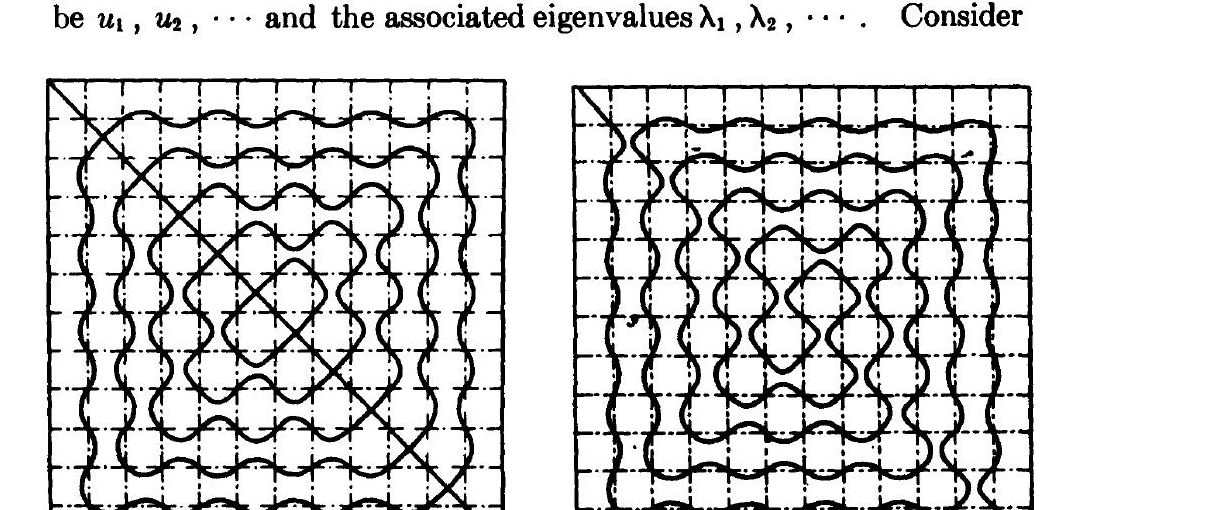
\includegraphics[width=0.92\textwidth]{figures/ch06_fig7_8.png}
\end{center}

any function $\varphi$ with continuous first derivatives and piecewise continuous second derivatives in $G$ which vanishes on the boundary $\Gamma$ and satisfies the conditions
\begin{equation}\tag{50}
\iint_G\rho\varphi^2\,dx\,dy=1,
\end{equation}
\begin{equation}\tag{51}
\iint_G\rho\varphi u_i\,dx\,dy=0\qquad(i=1,2,\ldots,n-1).
\end{equation}
We now show that $\varphi$ satisfies the inequality
\[
D[\varphi]\ge\lambda_n.
\]

% --- printed p.457 ---
For, because of the boundary condition $\varphi=0$, Green's formula yields
\[
D[\varphi]=-\iint_G\varphi L[\varphi]\,dx\,dy;
\]
in addition, the completeness relation (cf. formula (23a), page 426), applied to the functions $\varphi$ and $L[\varphi]/\rho$, leads to the relation
\begin{equation}\tag{52}
D[\varphi]=-
\sum_{i=1}^{\infty}\gamma_i\iint_Gu_iL[\varphi]\,dx\,dy,
\end{equation}
where
\[
\gamma_i=\iint_G\rho\varphi u_i\,dx\,dy.
\]
It follows from (52), with the aid of Green's formula and the relation $L[u_i]=-\lambda_i\rho u_i$, that
\begin{equation}\tag{53}
D[\varphi]=\sum_{i=1}^{\infty}\lambda_i\gamma_i^2.
\end{equation}
Now, since (51) implies
\[
\gamma_i=0\qquad\text{for }i=1,2,\ldots,n-1,
\]
and since from (50), together with the completeness relation, we have
\[
\sum_{i=1}^{\infty}\gamma_i^2=1,
\]
it follows immediately that if the $\lambda_i$ are ordered according to increasing magnitude, we have
\[
D[\varphi]\ge\lambda_n.
\]
Moreover, as shown earlier, by a simple calculation we obtain
\[
D[u_n]=\lambda_n,
\]
which means we have proved the minimizing property of the $n$-th eigenfunction with respect to the function $\varphi$. The same considerations may be applied if we assume only that the functions $\varphi$ are continuous and have piecewise continuous first derivatives; for, a function of this kind, together with its derivative, may always be approximated by a function of the class defined above in such a way that the corresponding integrals $D[\varphi]$ differ by an arbitrarily small amount (in this connection, see the remarks in Ch. IV, \S3, 7).

\subsection{Characterization of the First Eigenfunction by Absence of Nodes}
The first eigenfunction has been characterized by the property that it does not vanish. We shall now use an important method introduced by Jacobi to investigate this property (method of multiplicative variation).

We limit ourselves to the equation
\[
\Delta u-qu+\lambda u=0.
\]
We wish to prove: If there exists a solution $u$ of this equation which vanishes on the boundary $\Gamma$ of a domain $G$ but nowhere in the interior, then
\[
\mathfrak D[\varphi]=\iint_G(\varphi_x^2+\varphi_y^2+q\varphi^2)\,dx\,dy
\ge\lambda\iint_G\varphi^2\,dx\,dy
\]
for all admissible functions $\varphi$, where the equality holds only for $\varphi=\text{const}\times u$. We suppose every such function $\varphi$ to be represented in the form
\[
\varphi=u\eta,
\]
which is possible, since $u$ does not vanish in $G$; we have
\begin{align*}
\mathfrak D[\varphi]
={}&\iint_G\bigl[u^2(\eta_x^2+\eta_y^2)+2uu_x\eta\eta_x+2uu_y\eta\eta_y\\
&\hspace{36mm}+(u_x^2+u_y^2)\eta^2+qu^2\eta^2\bigr]dx\,dy.
\end{align*}
By observing $2\eta\eta_x=(\eta^2)_x$, $2\eta\eta_y=(\eta^2)_y$ and integrating by parts, we obtain
\[
\mathfrak D[\varphi]=\iint_G\bigl[u^2(\eta_x^2+\eta_y^2)-u\Delta u\,\eta^2+qu^2\eta^2\bigr]dx\,dy
\]
since all the integrals over the boundary vanish. Making use of the differential equation for $u$, we find
\[
\mathfrak D[\varphi]=\iint_G\bigl[u^2(\eta_x^2+\eta_y^2)+\lambda u^2\eta^2\bigr]dx\,dy
\ge\lambda\iint_Gu^2\eta^2\,dx\,dy
=\lambda\iint_G\varphi^2\,dx\,dy,
\]
where the equality holds only for $\eta_x=\eta_y=0$, i.e. for $\eta=\text{const.}$, q.e.d.

\subsection{Further Minimizing Properties of Eigenvalues}
The reader may prove the following theorem: The problem of minimizing the integral expression
\[
D[v_1,v_2,\ldots,v_n]
=\mathfrak D[v_1]+\mathfrak D[v_2]+\cdots+\mathfrak D[v_n],
\]
in which we admit all systems of $n$ mutually orthogonal normalized functions with piecewise continuous derivatives in the fundamental domain $G$, is solved by the functions $v_i=u_i$ or by any system of functions which arise from these functions through an orthogonal transformation. Here the functions $u_1,u_2,\ldots,u_n$ stand for the first $n$ eigenfunctions for the domain. The minimum of $D[v_1,v_2,\ldots,v_n]$ is equal to the sum of the first $n$ eigenvalues, $\lambda_1+\lambda_2+\cdots+\lambda_n$.

The following theorem can also be proved: Let $v_1,v_2,\ldots,v_{n-1}$ be continuous functions in $G$, and let $d(v_1,v_2,\ldots,v_{n-1})$ be the lower bound of the integral expression $\mathfrak D[\varphi]$ where, in addition to satisfying the usual continuity conditions, $\varphi$ is subject to the single auxiliary condition
\[
\iint_G\rho\varphi^2\,dx\,dy
-\sum_{i=1}^{n-1}\left(\iint_G\rho\varphi v_i\,dx\,dy\right)^2=1.
\]
Then the $n$-th eigenvalue $\lambda_n$ equals the maximum of $d(v_1,v_2,\ldots,v_{n-1})$ and is assumed for $v_1=u_1,v_2=u_2,\ldots,v_{n-1}=u_{n-1};\ \varphi=u_n$.

This formulation is interesting since it uses only one quadratic auxiliary condition and does not require linear conditions; however, the auxiliary condition has a form which is unusual for isoperimetric problems. It will be left as a problem for the reader to carry over this formulation to the corresponding elementary problem for quadratic forms.

Other formulations of the eigenvalue problems, useful in many applications, will be given in connection with the differential equation $\Delta u+\lambda u=0$ with the boundary condition $u=0$:
\[
H[\varphi]=\iint_G\varphi^2\,dx\,dy=\min.\max.
\]
subject to the auxiliary conditions
\[
D[\varphi]=\iint_G(\varphi_x^2+\varphi_y^2)\,dx\,dy=1,
\qquad
D[\varphi,v_i]=0\quad(i=1,2,\ldots,n-1),
\]
from which one sees immediately the significance of the formulation as a maximum-minimum problem.

Another equivalent problem is that of making the expression
\[
\iint_G(\Delta\varphi)^2\,dx\,dy
\]
a maximum-minimum under the same auxiliary conditions, where we again require the functions $\varphi$ to have continuous first and piecewise continuous second derivatives.

\subsection{Asymptotic Distribution of Eigenvalues}
(a) For the differential equation $\Delta\Delta u-\lambda u=0$ of the vibrating plate, with the boundary conditions $u=0$ and $\partial u/\partial n=0$ (clamped plate), we have the asymptotic relation
\[
A(\lambda)\sim\frac{f}{4\pi}\sqrt\lambda,
\]
from which
\[
\lambda_n\sim\left(\frac{4\pi n}{f}\right)^2
\]
follows. Here, as earlier, $A(\lambda)$ is the number of eigenvalues less than the bound $\lambda$, $\lambda_n$ denotes the $n$-th eigenvalue, and $f$ the area of the plate. We may state, therefore: The $n$-th eigenvalue of the clamped plate, as $n$ increases, is asymptotically equal to the square of the $n$-th eigenvalue of the clamped membrane. In particular, it depends only on the size and not on the shape of the plate. An analogous statement holds in three dimensions.\footnote{See Courant, Über die Schwingungen eingespannter Platten.}

(b) Derive the laws of asymptotic distribution of eigenvalues for the Sturm-Liouville equation (see the results of \S2, 3) and also for ordinary differential equations of fourth order, using the methods of \S4, 3.

(c) Derive the laws of the asymptotic distribution of eigenvalues for the case of elliptic self-adjoint differential equations arising from an arbitrary definite quadratic variational problem.

\subsection{Parameter Eigenvalue Problems}
Carry out the solution of two-parameter eigenvalue problems (see the Lamé problem in Ch. V, \S9, 3) using methods of the calculus of variations.

\subsection{Boundary Conditions containing Parameters}
Eigenvalue problems with the parameter in the boundary condition (cf. Ch. V, \S16, 4) may also be solved easily with the aid of methods of the calculus of variations. For the differential equation $\Delta u=0$ and the boundary condition $\partial u/\partial n=\lambda u$, we have to minimize an integral of the form
\[
\iint_G(\varphi_x^2+\varphi_y^2)\,dx\,dy
\]
where the integral of $\varphi^2$ over the boundary satisfies the condition
\[
\int_\Gamma\varphi^2\,ds=1
\]
and suitable linear auxiliary conditions are imposed. Further development of this idea is left to the reader.

If $G$ is the unit circle, the solutions of this problem are given by the potential functions $r^n\cos n\theta$, $r^n\sin n\theta$; the eigenvalues are $\lambda_n=n$.

In the general case, it is easily seen with the aid of the methods developed in the present chapter that $\lambda_n$ is of the order of $n$. It therefore follows from \S3, 1 that the eigenfunctions are complete with respect to the expression
\[
\mathfrak H[\varphi]=\int_\Gamma\varphi^2\,ds.
\]
In other words, the boundary values of the eigenfunctions considered as functions of $s$ form a complete system from which, in turn, it may be concluded that every potential function which is regular in $G$ may be approximated in the mean by its eigenfunctions.

\subsection{Eigenvalue Problems for Closed Surfaces}
The eigenvalue problem of the Laplace spherical harmonics is an example of a problem on a closed surface, for which the condition of regularity over the entire surface replaces boundary conditions. The methods of the present chapter show that these eigenvalue problems are closely related to minimum or to maximum-minimum problems for a quotient $\mathfrak D/\mathfrak H$; $\mathfrak D$ is a quadratic expression formed with the derivatives of $\varphi$ and $\mathfrak H[\varphi]$ is a positive definite quadratic expression which does not contain derivatives and has the closed surface as the domain of integration. This theory may be carried over to other quadratic differential expressions on closed surfaces.

\subsection{Estimates of Eigenvalues when Singular Points Occur}
In \S2, 4 we treated singular points in connection with Bessel eigenvalue problems; Bessel functions of zero-th order required special treatment using particular properties of the Bessel functions. This will no longer be necessary because we shall now develop a more general method.

We consider the eigenvalue problem associated with the expressions
\[
D[\varphi]=\int_0^1x\varphi'^2\,dx,
\qquad
H[\varphi]=\int_0^1x\varphi^2\,dx
\]
with no boundary conditions at $x=0$, and with the boundary condition $\varphi(1)=0$ at $x=1$. After introducing $\sqrt x\,\varphi$ as new dependent variable, we find without difficulty the estimate $\lambda_n<n^2\pi^2$ for the $n$-th eigenvalue $\lambda_n$ of our problem. Thus for the number $A(\lambda)$ of eigenvalues less than $\lambda$ we have $A(\lambda)\ge\sqrt\lambda/\pi$.

In order to estimate $\lambda_n$ from below, and thus find an upper bound for $A(\lambda)$---this is our specific objective here---we choose an arbitrarily small positive number $\epsilon$ between 0 and 1 and note that $A(\lambda)\le B_1(\lambda)+B_2(\lambda)$, where $B_1$ and $B_2$ denote the number of eigenvalues less than $\lambda$ of the expressions
\[
D_1=\int_0^\epsilon x\varphi'^2\,dx,
\qquad
H_1=\int_0^\epsilon x\varphi^2\,dx
\]
and
\[
D_2=\int_\epsilon^1 x\varphi'^2\,dx,
\qquad
H_2=\int_\epsilon^1 x\varphi^2\,dx,
\]
respectively. Here we no longer require that the function $\varphi$ be continuous at the point $x=\epsilon$, so that in both cases the point $x=\epsilon$ occurs as a free end point. Using the methods developed in this chapter we find the asymptotic relation $B_2(\lambda)/\sqrt\lambda\to(1-\epsilon)/\pi$ for $B_2(\lambda)$; it remains to estimate $B_1(\lambda)$. We majorize $H_1$ by $H_1^*$ and minorize $D_1$ by $D_1^*$:
\[
H_1^*=\epsilon\int_0^\epsilon\varphi^2\,dx,
\qquad
D_1^*=\int_0^\epsilon x\left(1-\frac{x}{\epsilon}\right)\varphi'^2\,dx.
\]
Using an obvious notation, we have $B_1(\lambda)<B_1^*(\lambda)$. On the other hand, we can write down the eigenfunctions and eigenvalues of this new eigenvalue problem explicitly. To do this, we map the interval $0\le x\le\epsilon$ onto the interval $-1\le\xi\le1$ by the transformation
\[
x=\frac{(1+\xi)\epsilon}{2}.
\]
For the eigenfunctions we obtain the Legendre polynomials in $\xi$, and for the eigenvalues the numbers $n(n+1)/\epsilon^2$. Hence $B_1(\lambda)\le B_1^*(\lambda)\le\epsilon(1+\delta)\sqrt\lambda$, where $\delta$ approaches zero with increasing $\lambda$. Summing up our results, we obtain almost immediately the asymptotic relation
\[
\lim_{\lambda\to\infty}\frac{A(\lambda)}{\sqrt\lambda}=\frac1\pi
\]
since $\epsilon$ could be chosen arbitrarily small.

\subsection{Minimum Theorems for the Membrane and Plate}
Of all clamped membranes or plates with given perimeter or area and given constant density and elasticity, those with the circle as boundary have the lowest fundamental tone. (For proofs, see the first paper cited below for the case of a given constant perimeter, and the works of G. Faber\footnote{G. Faber, Beweis, dass unter allen homogenen Membranen von gleicher Fläche und gleicher Spannung die kreisförmige den tiefsten Grundton gibt, S.-Ber. Bayr. Akad. Wiss. (math.-phys. Kl.), 1923, pp. 169--172.} and E. Krahn\footnote{E. Krahn, Über eine von Rayleigh formulierte Minimaleigenschaft des Kreises, Math. Ann., Vol. 94, 1925, pp. 97--100.} for the case of a given constant area.)

\subsection{Minimum Problems for Variable Mass Distribution}
The reader may prove the following theorems:

The fundamental tone of a stretched string of given uniform tension along which a given mass has been distributed is lowest when the entire mass is concentrated at the midpoint.

Prove the analogous results for the membrane and plate.

\subsection{Nodal Points for the Sturm-Liouville Problem. Maximum-minimum Principle}
The theorem of \S6, which states that the $n$-th eigenfunction divides the fundamental domain into $n$ parts by means of its zeros, can also be proved on the basis of the following considerations.\footnote{See K. Hohenemser, Praktische Wege zur angenäherten Schwingungsberechnung elastischer Systeme. Ingenieur-Archiv, Vol. 1, No. 3, 1930, pp. 1--24.} Given a string capable of vibrating, if $n-1$ arbitrarily chosen inner points are fixed, the fundamental tone of the resulting system consisting of $n$ independent strings is identical with the lowest of the fundamental tones of the subsystems (see \S1, 3). The fundamental vibration of the decomposed system is then the fundamental vibration of the subsystem in question while the remaining subsystems are constrained to the rest position. If we vary the prescribed nodal points, the fundamental tone of the decomposed system reaches a maximum when the $n$ subsystems all have the same fundamental tone. For, if two neighboring subsystems had different fundamental tones, we could raise the fundamental tone of one and lower that of the other by moving the nodal point which they have in common so that both subsystems would have equally high fundamental tones. Now, in the extremal case considered, the fundamental vibration of the decomposed system may be represented by a continuously differentiable function which represents an eigenfunction of the original unrestrained system associated with the vibration frequency in question and vanishing at the $n-1$ points corresponding to the maximum fundamental tone. Hence: \emph{If a string is fixed at $n-1$ points, and we wish to choose these points in such a way that the fundamental tone of the resulting system is as high as possible, we find that the solution is given by an eigenfunction of the original system having $n-1$ zeros at inner points.} If we call the eigenvalues thus obtained $\mu_n$ and the associated eigenfunctions $v_n$, then $\mu_{n+1}\ge\mu_n$, since there exists an interval, determined by two suitably neighboring zeros of $v_n$, which contains the interval between two zeros of $v_{n+1}$ as a proper subinterval, and since a reduction in the length of the interval produces a rise in the fundamental tone. (See page 455, footnote.)

If, as before, we denote the eigenvalues of the string, ordered with respect to increasing magnitude, by $\lambda_n$, we see that we always have $\mu_n\ge\lambda_n$ since the $\mu_n$ must certainly be contained among the $\lambda_n$. On the other hand, the restriction of a prescribed nodal point is only a special or limiting case of a linear auxiliary condition such as we have considered in \S1, 4 for the variational problems defining the eigenvalues $\lambda_n$. If we limit ourselves to such special auxiliary conditions the maximum-minimum, i.e. the number $\mu_n$, cannot be greater than the maximum of the minimum when arbitrary linear auxiliary conditions are admitted, i.e. not greater than $\lambda_n$. Hence $\mu_n\le\lambda_n$, and therefore, in view of the above result, we have $\mu_n=\lambda_n$. This completes the proof of the theorem on the zeros of Sturm-Liouville eigenfunctions.

\begin{center}
\textbf{References}
\end{center}
\noindent Courant, R., Beweis des Satzes, dass von allen homogenen Membranen gegebenem Umfanges und gegebener Spannung die kreisförmige den tiefsten Grundton besitzt. Math. Zeitschr., Vol. 1, 1918, pp. 321--328.\\
---, Über die Eigenwerte bei den Differentialgleichungen der mathematischen Physik. Ibid., Vol. 7, 1920, pp. 1--57.\\
---, Über die Schwingungen eingespannter Platten. Ibid., Vol. 15, 1922, pp. 195--200.\\
---, Ein allgemeiner Satz zur Theorie der Eigenfunktionen selbstadjungierter Differentialausdrücke. Nachr. Ges. Göttingen (math.-phys. Kl.), 1923, Session of July 13.\\
---, Über die Anwendung der Variationsrechnung in der Theorie der Eigenschwingungen und über neue Klassen von Funktionalgleichungen. Acta Math., Vol. 49, 1926, pp. 1--68.\\
Kneser, A., Die Integralgleichungen und ihre Anwendungen in der mathematischen Physik. 2nd ed., F. Vieweg und Sohn, Braunschweig, 1922.\\
Liouville, J., Mémoire sur le développement des fonctions ou parties de fonctions en séries dont les divers termes sont assujettis à satisfaire à une même équation différentielle du second ordre contenant un paramètre variable. J. de math. pures et appl., Ser. 1, Vol. 1, 1836, pp. 253--265. Ibid., Vol. 2, 1837, pp. 16--35, 418--436.\\
Weyl, H., Das asymptotische Verteilungsgesetz der Eigenwerte linearer partieller Differentialgleichungen (mit einer Anwendung auf die Theorie der Hohlraumstrahlung). Math. Ann., Vol. 71, 1912, pp. 441--479.\\
---, Über die Abhängigkeit der Eigenschwingungen einer Membran von deren Begrenzung. Journ. f. d. reine u. angew. Math., Vol. 141, 1912, pp. 1--11.\\
---, Über das Spektrum der Hohlraumstrahlung. Ibid., pp. 163--181.\\
---, Über die Randwertaufgabe der Strahlungstheorie und asymptotische Spektralgesetze. Ibid., Vol. 143, 1913, pp. 177--202.\\
Richardson, R. G. D., Das Jacobische Kriterium der Variationsrechnung und die Oszillationseigenschaften linearer Differentialgleichungen zweiter Ordnung. First communication, Math. Ann., Vol. 68, 1910, p. 279. Second communication, Ibid., Vol. 71, 1911--12, p. 214.\\
---, Über die notwendigen und hinreichenden Bedingungen für das Bestehen eines Kleinschen Oszillationstheorems. Ibid., Vol. 73, 1913, p. 289.\\[0.4em]
In an unpublished manuscript, submitted in 1914 to the editors of Mathematische Annalen in the form of an abstract, Richardson treated the eigenvalue problem of elliptic differential equations with results similar to some of those of the present chapter. In particular, Richardson's paper dealt with the behavior of the eigenvalues and the coefficients in the boundary condition with respect to the growth of the domain and their independence of the coefficients of the differential equation; he also treated theorems concerning the zeros of the eigenfunctions.
